\documentclass[11pt,aspectratio=169]{beamer}

% --- Tema og fonte ---
\usetheme{Madrid}
\usefonttheme{serif}
% --- Farver ---
\definecolor{myteal}{RGB}{14,71,57}
\setbeamercolor{title}{fg=white}
\setbeamercolor{frametitle}{fg=white,bg=myteal}
\setbeamercolor{block title}{fg=white,bg=myteal}
\setbeamercolor{block body}{bg=myteal!10}
\setbeamercolor{normal text}{fg=myteal}
\setbeamercolor{background canvas}{bg=white}
\setbeamercolor{structure}{fg=myteal}
\setbeamercolor{palette primary}{fg=white,bg=myteal}
\setbeamercolor{palette secondary}{fg=white,bg=myteal!80}
\setbeamercolor{palette tertiary}{fg=white,bg=myteal!60}
\setbeamercolor{author in head/foot}{fg=white,bg=myteal}
\setbeamercolor{title in head/foot}{fg=white,bg=myteal!80}
\setbeamercolor{date in head/foot}{fg=white,bg=myteal!60}
\setbeamercolor{titlelike}{fg=myteal}
\setbeamercolor{section in toc}{fg=myteal}
\setbeamercolor{item}{fg=myteal}
% --- Sprog og encoding ---
\usepackage[utf8]{inputenc}
\usepackage[danish]{babel}
\usepackage[T1]{fontenc}
\usepackage{lmodern}
% --- Matematik ---
\usepackage{amsmath,amsfonts,amssymb}
% --- Grafik og layout ---
\usepackage{graphicx}
\usepackage{ragged2e}
\usepackage{booktabs}
\usepackage{arydshln}
\usepackage[most]{tcolorbox}
% --- Ikoner og figurer ---
\usepackage{fontawesome5}
\usepackage{tikz}
\usetikzlibrary{positioning,arrows.meta,shapes.geometric,calc}
\usepackage{circuitikz}
% --- Positionering ---
\usepackage[absolute,overlay]{textpos}
% --- CSV ---
\usepackage{csvsimple}
% --- Kildehenvisning nederst på slides ---
\setbeamercolor{framesource}{fg=gray,bg=white}
\setbeamerfont{framesource}{size=\scriptsize}
\newcommand{\framesource}[1]{%
  \begin{textblock*}{12cm}(0.5cm,8.6cm)
    \raggedleft
    \beamercolorbox[wd=\textwidth,rightskip=0.5cm]{framesource}{#1}
  \end{textblock*}
}
% --- Automatisk billedattribution ---
\csvreader[
  head to column names,
  no head
]{Billeder/billedkilder.csv}{}{}
\newcommand{\billedkilde}[1]{%
  \csvreader[
    head to column names,
    full filter=\ifcsvstrcmp{\filnavn}{#1}{\csvfilteraccept}{\csvfilterreject},
    no head
  ]{Billeder/billedkilder.csv}{}%
  {%
    \tiny\forfatter\ / Wikimedia Commons (\licens)%
  }%
}
% --- Boksstile til jagttid-sliden ---
\tcbset{
  gruppe/.style={
    enhanced,
    colback=white,
    colframe=myteal,
    coltitle=myteal,
    boxrule=0.8pt,
    dashed,
    sharp corners,
    fonttitle=\bfseries\large,
    attach boxed title to top left={yshift=-2mm,xshift=3mm},
    boxed title style={colback=white,colframe=white,boxrule=0pt,sharp corners},
    top=1mm,left=1mm,right=1mm,bottom=1mm
  },
  felt/.style={
    enhanced,
    colback=white,
    colframe=myteal,
    boxrule=0.6pt,
    sharp corners,
    halign=center,
    valign=center,
    width=\linewidth,
    height=1.55cm,
    fit,
    fit algorithm=fontsize,
    fit basedim=7pt,
    boxsep=0.3mm,
    left=0.5mm, right=0.5mm, top=0.3mm, bottom=0.3mm
  },
  feltfri/.style={
    enhanced,
    colback=white,
    colframe=myteal,
    boxrule=0.6pt,
    sharp corners,
    halign=center,
    valign=center,
    width=\linewidth,
    boxsep=0.3mm,
    left=0.5mm, right=0.5mm, top=0.3mm, bottom=0.3mm,
    fontupper=\scriptsize
  }
}
% --- Matematiske operatorer ---
\DeclareMathOperator{\sen}{sen}
\DeclareMathOperator{\tg}{tg}
% --- Beamer-indstillinger ---
\setbeamertemplate{caption}[numbered]
\setbeamertemplate{navigation symbols}{}
% --- Forfatter ---
\author[Østerbro Jagttegn]{Østerbro Jagttegn \\ \textbf{Aleksander Sønder}}
% --- Hyperref (altid sidst) ---
\usepackage{hyperref}
\hypersetup{
  colorlinks=true,
  linkcolor=myteal,
  urlcolor=myteal,
  citecolor=myteal
}

\title{Obligatorisk Teori 1 \\
Hold Flex 26}
\date{\today}

\begin{document}

% Titelside
\begin{frame}
  \titlepage
\end{frame}

% Indholdsfortegnelse (valgfri)
\begin{frame}{Program}
  \tableofcontents
\end{frame}

\section{Introduktion}

\begin{frame}{Introduktion}
  \begin{columns}[T]
    % Venstre kolonne (55% af bredden)
    \column{0.55\textwidth}
    \hspace*{1cm}
    \begin{minipage}{0.85\textwidth}
      \small
      \setlength{\parskip}{0.1cm} % Reduceret linjeafstand
      \RaggedRight
      \textbf{\large Aleksander Sonder} \par
      \vspace{0.05cm} % Minimal luft før sektioner
      \textbf{Jagterfaring} \par
      Jagttegn siden 1997 \par
      Jagttegnslærer \par
      Skydeinstruktør \par
      Riffel og haglgevær \par
      Hundefører \par
      \vspace{0.05cm} % Minimal luft før sektioner
      \textbf{Privat} \par
      Familiefar \par
      \vspace{0.05cm}
      \textbf{Professionelt} \par
      Selvstændig, bestyrelse mm \par
      \vspace{0.05cm}
      \textbf{Uddannelse} \par
      DTU, RUC mm \par
    \end{minipage}
    
    % Højre kolonne (45% af bredden)
    \column{0.45\textwidth}
    \centering
    \vspace*{0.4cm} % Lidt mindre vertikal plads øverst
    \fbox{
      
\includegraphics[width=0.7\textwidth]{Billeder/Andet/AKSS.jpg}
    }
    \vspace*{0.2cm} % Mindre plads under billedet
  \end{columns}
\end{frame}

\begin{frame}{Lidt om jer?}
  \begin{columns}[T]
    % Venstre kolonne (55% af bredden) – spørgsmål med bullets
    \column{0.55\textwidth}
    \hspace*{1cm}
    \begin{minipage}{0.85\textwidth}
      \small
      \setlength{\parskip}{0.1cm}
      \RaggedRight
      \begin{itemize}
        \item \large Navn?
        \item \large Hvorfor vil du tage jagttegn?
        \item \large Har du været med på jagt?
        \item \large Har du prøvet at skyde?
      \end{itemize}
    \end{minipage}
    
    % Højre kolonne (45% af bredden) – ikon
    \column{0.45\textwidth}
    \centering
    \vspace*{0.4cm} % Justerer lodret placering
    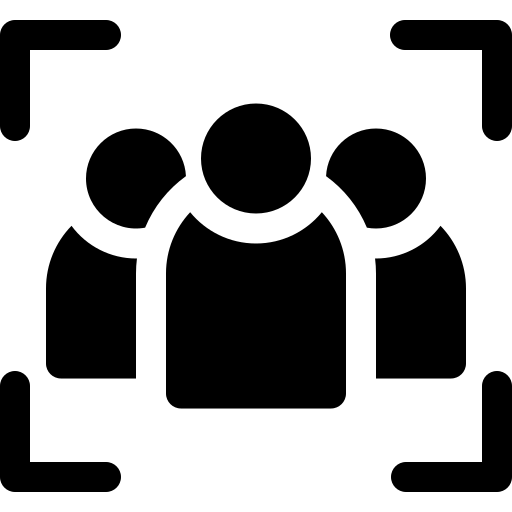
\includegraphics[width=0.50\textwidth]{Billeder/Andet/target-audience.png}
  \end{columns}
\end{frame}

\begin{frame}{Formalia}
  \vspace{1em}
  \begin{columns}[T]
    \column{0.05\textwidth}
    \column{0.9\textwidth}
    \setlength{\parskip}{0.4em}
    \small
    \RaggedRight

    \textbf{JægerID:} \\
    \url{https://sgavmst.dk/natur-og-jagt/jagttegn/jagttegnsaspirant} \par

    \vspace{0.5em}
    \textbf{Simulerede teoriprøver:} \\
    \url{https://osjagttegn.dk/} (gratis)\\
    \url{https://jagtproeven.dk/} (100  kr) \par

    \vspace{0.5em}
    \textbf{Google Drive (præsentationer mm):} \\
    \url{https://drive.google.com/drive/folders/1iLtHqLLlpJ-f5kI5OEOSgUxoz1dal9t4?usp=sharing } \par

    \vspace{0.5em}
    \textbf{WhatsApp (chat/feedback):} \\
    \url{https://chat.whatsapp.com/BMfd13gMv2RL8rK3jt25jy} \par

    \column{0.05\textwidth}
  \end{columns}
\end{frame}

\begin{frame}{Våbenhåndtering og sikkerhedsregler}
  \vspace{1em}
  \begin{columns}[c] % c = center vertically
    \column{0.05\textwidth} % Venstre margin (kan fjernes eller justeres)

    \column{0.7\textwidth} % Midten: Bullets
    \small
    \raggedright

    \begin{itemize}
      \itemsep0.6em % Justér afstand mellem bullets
      \item Brug alle muligheder for at øve våbenhåndtering (tørtræning) med haglgevær.
      \item Våben må \alert{ikke} forlade kursuslokalet/gangen.
      \item Våben må \alert{kun} håndteres i Aleksanders nærvær.
      \item Brug \alert{altid} klikpatroner.
    \end{itemize}

    \column{0.25\textwidth} % Højre: Ikon (størrelsen tilpasses her)
    \centering
    \vspace{0pt} % hjælper med vertikal centring i nogle temaer
    
\includegraphics[width=0.8\linewidth]{Billeder/Andet/shotgun.png}

  \end{columns}
\end{frame}

\begin{frame}{Materiale}
  \vspace{1em}
  \begin{columns}[T]
    \column{0.05\textwidth}

    \column{0.9\textwidth}
    \setlength{\parskip}{0.4em}
    \small
    \RaggedRight

    \textbf{Jagttegn – 6. udgave:} \\
    Niels Søndergård, ISBN 978-87-93976-28-3 \\
    \url{https://netbutikken.seges.dk/index.php/jagt/jagttegn-541.html} \par

    E-bog/PDF version: \\
    \url{https://jagtproeven.dk/materialer/boger/} \par

    \vspace{0.5em}
    \textbf{Supplerende:} \\[0.2em]
    Lovsamling til jægeren 2024–2025 \\
    \url{https://netbutikken.seges.dk/index.php/jagt/lovsamling-til-jaegeren-2024-25.html} \par

    Wildcards \\
    \url{https://netbutikken.seges.dk/index.php/jagt/wildcards.html} \par

    Fuglekort \\
    \url{https://www.fuglekort.com/} \par

    \column{0.05\textwidth}
  \end{columns}
\end{frame}

\begin{frame}{Teoriemner}
\begin{itemize}
    \item Artsbestemmelse
    \item Vildtforvaltning
    \item Jagtvåben og ammunition
    \item Jagtlovgivning
    \item Håndtering af nedlagt vildt
    \item Jagtetik og -etikette
    \item Jagtteknik og -ledelse
    \item Skudafgivelse med forskellige våben
\end{itemize}
\end{frame}

\begin{frame}{Lektionsplan}
  \vspace{1em}
  \begin{columns}[T]
    \column{0.05\textwidth}

    \column{0.9\textwidth}
    \setlength{\parskip}{0.4em}
    \small
    \RaggedRight

    \textbf{Lektionsplan}

    \column{0.05\textwidth}
  \end{columns}
\end{frame}


\begin{frame}
  \vspace{3em}
  \begin{center}
    {\LARGE \textbf{Jagtprøven}}
  \end{center}
\end{frame}



\section{Jagtprøven}

\begin{frame}{Jagtprøven – teoretisk del}
  \vspace{0.8em}
  \begin{columns}[T]
    \column{0.05\textwidth}

    \column{0.9\textwidth}
    \setlength{\parskip}{0.4em}
    \footnotesize
    \RaggedRight

    Teoretisk prøve skal bestås \textbf{før} praktisk prøve kan aflægges \par

    40 spørgsmål – \textbf{maks. 4 fejl} \par

    30 min. uden hjælpemidler (\textbf{45 sek. pr. spørgsmål}) \par

    Multiple choice i forskellige variationer \par

    \vspace{0.3em}
    \textbf{Emner (antal spørgsmål):} \\
    Jagtlovgivning (13), Vildtkendskab (10), \\
    Vildtbiologi/jagt/vildtforvaltning (8), \\
    Jagtvåben/ammunition (3), \\
    Etik/jagtteknik/jagtledelse (3), \\
    Sikkerhed (3) \par

    \vspace{0.3em}
    \textbf{3 forsøg} \par

    \vspace{0.2em}
    \textit{Bestås teoriprøven, men dumpes den praktiske prøve, \\
    skal teoriprøven \textbf{ikke} aflægges igen inden for de 3 forsøg.} \par

    \column{0.05\textwidth}
  \end{columns}
\end{frame}

\begin{frame}{Jagtprøven – praktisk del}
  \vspace{1em}
  \begin{columns}[T]
    \column{0.05\textwidth}

    \column{0.9\textwidth}
    \setlength{\parskip}{0.5em}
    \small
    \RaggedRight

    Sikker håndtering af haglgevær \par

    Sikker forcering af forhindringer (hegn/grøft) \par

    6 afstandsbedømmelser til vildtfigurer (\textbf{maks. 1 fejl}) \par

    Sikker afgivelse af skud til lerduer (bagduer) – \\
    \textit{ikke et krav at ramme!} \par

    \vspace{0.4em}
    \textbf{3 forsøg} \par

    \vspace{0.3em}
    \textit{Bestås praktisk prøve ikke, må teoriprøven \\
    \textbf{beholdes} inden for de 3 forsøg.} \par

    \column{0.05\textwidth}
  \end{columns}
\end{frame}

\begin{frame}{Praktisk prøve - visualisering}
    \centering
    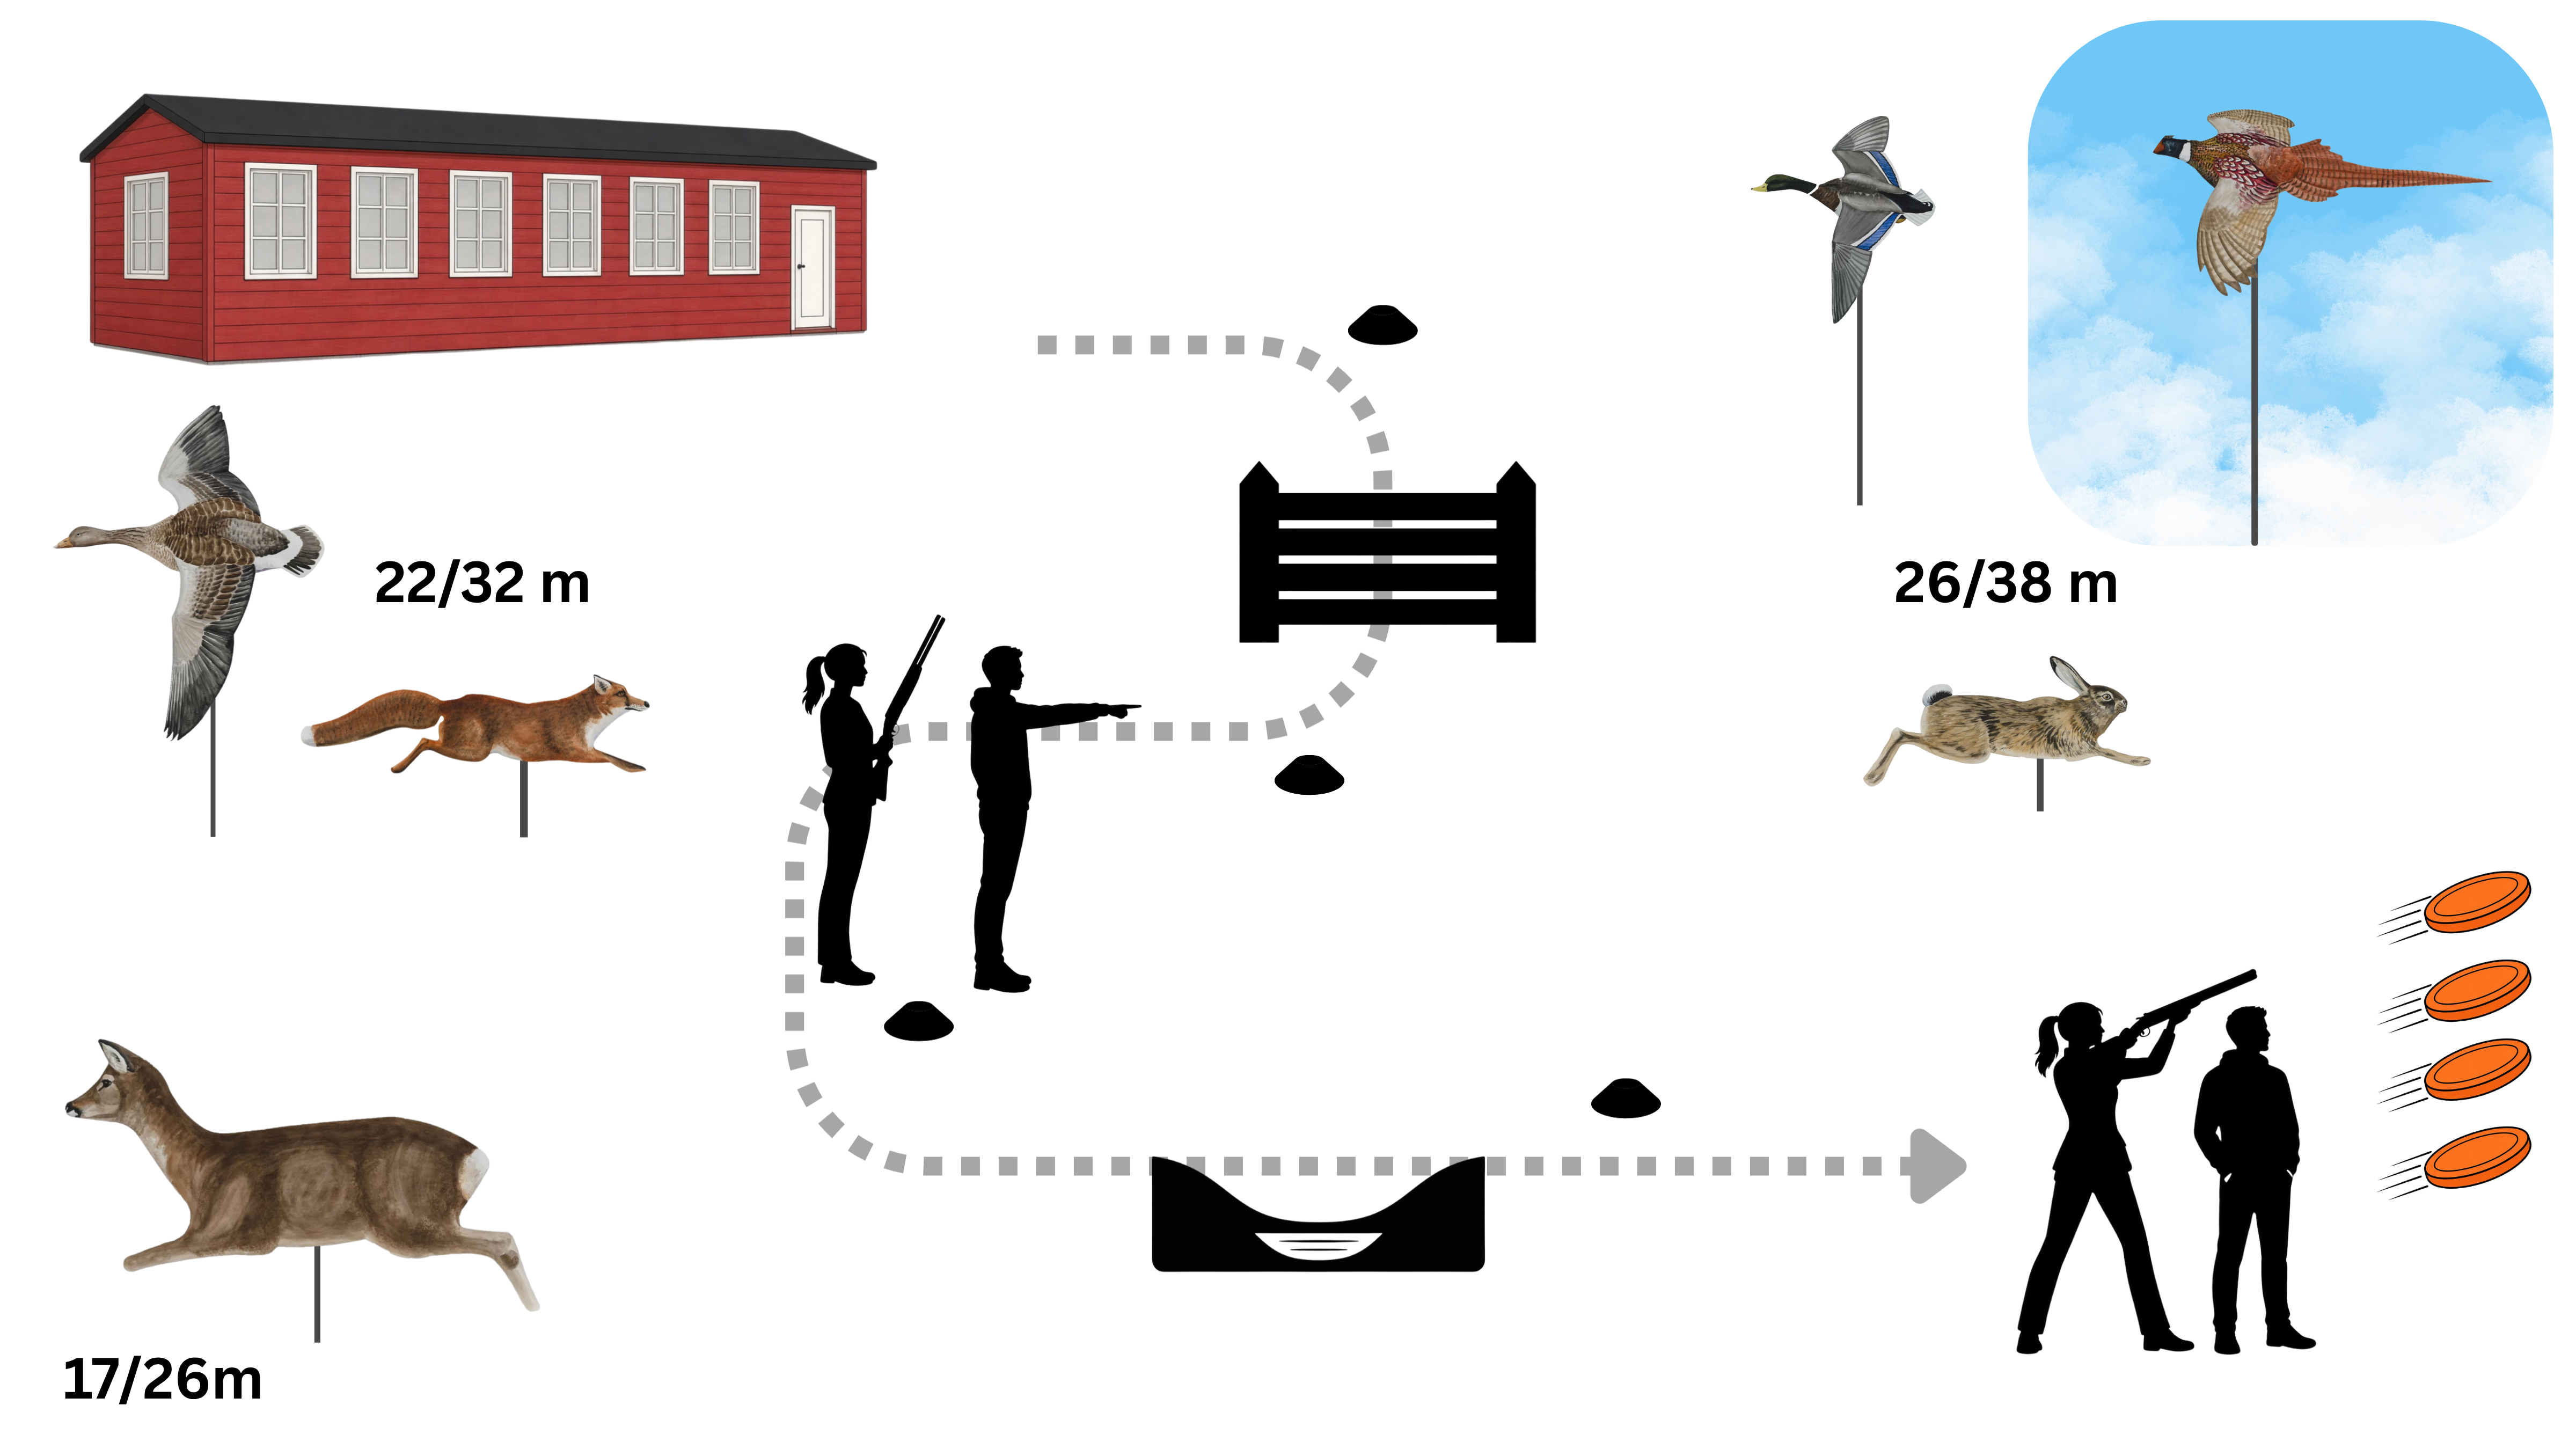
\includegraphics[width=0.85\textwidth]{Billeder/Andet/2638 m (1).png}
\end{frame}

\begin{frame}{Vejen til jagttegn}
\centering
\resizebox{0.85\textwidth}{!}{%
\begin{figure}[!ht]
\centering
\begin{circuitikz}
\tikzstyle{every node}=[font=\Large]

% Obligatorisk jagttegnskursus
\draw [rounded corners=7.8] (11.5,18.5) rectangle node {\Large Obligatorisk jagttegnskursus} (20.5,16.5);

% Jagttegnsprøven
\draw [rounded corners=7.8] (13,15) rectangle node {\Large Jagttegnsprøven} (19,13.5);
\draw [->, >=Stealth] (16,16.5) -- (16,15);

% Jagttegn
\draw [rounded corners=7.8] (13,12) rectangle node {\Large Jagttegn} (19,10.5);
\draw [->, >=Stealth] (16,13.5) -- (16,12);

% De fire prøver
\draw [rounded corners=7.8] (2.5,8.5) rectangle node {\Large Haglskydeprøve} (8.5,7);
\draw [rounded corners=7.8] (9.5,8.5) rectangle node {\Large Riffelprøve} (15.5,7);
\draw [rounded corners=7.8] (16.5,8.5) rectangle node {\Large Bueprøve} (22.5,7);
\draw [rounded corners=7.8] (23.5,8.5) rectangle node {\Large Falkonerprøve} (29.5,7);

\draw [->, >=Stealth] (16,10.5) -- (5.5,8.5);
\draw [->, >=Stealth] (16,10.5) -- (12.5,8.5);
\draw [->, >=Stealth] (16,10.5) -- (19.5,8.5);
\draw [->, >=Stealth] (16,10.5) -- (26.5,8.5);

% Påtegning
\draw [rounded corners=7.8] (13,5) rectangle node {\Large Påtegning til jagttegn} (19,3.5);
\draw [->, >=Stealth] (5.5,7) -- (16,5);
\draw [->, >=Stealth] (12.5,7) -- (16,5);
\draw [->, >=Stealth] (19.5,7) -- (16,5);
\draw [->, >=Stealth] (26.5,7) -- (16,5);

\end{circuitikz}
\end{figure}
}%
\end{frame}

\section{1/2 teoriprøve}

\begin{frame}
  \vspace{3em}
  \begin{center}
    {\LARGE \textbf{1/2 Teoriprøve}}
  \end{center}
\end{frame}

\section{Våbenhåndtering}

\begin{frame}
  \vspace{3em}
  \begin{center}
    {\LARGE \textbf{Våbenhåndtering}}
  \end{center}
\end{frame}



\begin{frame}{Våbenhåndtering – trin for trin}
  \vspace{0.3em} % Mindsket plads
  \begin{columns}[T]
    % --- Venstre kolonne: Opstart + Forhindring (Originalt indhold) ---
    \column{0.48\textwidth}
    \setlength{\parskip}{0.28em} % Mindsket afstand mellem afsnit
    \footnotesize
    \RaggedRight

    \textbf{-- Opstart --} \\
    1. Fødder i skudretning – fri for mennesker. \\
    2. Forskæfte med \textit{modsatte hånd} af skulderen du vil lægge geværet til. \\
    3. Åbn geværet lodret med topnøgle. \\
    4. Kig igennem – \textit{tomt og rent}. \\
    5. Før gennem vandret (knækket). \\
    6. Isæt patroner. \\
    7. Luk i \textbf{45°} – hør \textit{klik}. \\
    8. Før op til \textit{semi-klar}. \\
    9. \textit{Fingre væk} fra aftrækker/sikring. \par

    \vspace{0.3em} % Mindsket plads
    \textbf{-- Forhindring --} \\
    10. Før geværet ned gennem vandret. \\
    11. Åbn – patroner \textit{i lommen}. \\
    12. Forcer med \textit{knækket gevær}. \\
    13. Efterse løbene. \\
    14. Isæt patroner igen. \\
    15. Før op gennem vandret. \par

    % --- Højre kolonne: Skudafgivelse (Originalt indhold) ---
    \column{0.48\textwidth}
    \setlength{\parskip}{0.28em} % Mindsket afstand mellem afsnit
    \footnotesize
    \RaggedRight

    \textbf{-- Skudafgivelse --} \\
    16. Geværet lades \\
    17. Op til \textit{semi-klar}. \\
    18. Kolbe mod bryst – nær armhule. Min 30° \\
    19. Meld: \textbf{„KLAR!“} \\
    20. Afsikring \textit{frem}. \\
    21. Affyr 1–2 skud. \\
    22. Ned til bryst. \\
    23. Sikring \textit{tilbage}. \\
    24. Ned gennem vandret. \\
    25. Åbn – fjern afskudte. \\
    26. Gentag \textbf{4 gange}. \\
    27. Aflever \textit{alle patroner}. \par

  \end{columns}
\end{frame}

\section{Jagttidsbekendtgørelsen}

\begin{frame}
  \vspace{3em}
  \begin{center}
    {\LARGE \textbf{Jagttidsbekendtgørelsen}}
    \vspace{2em}
    \\ Bekendtgørelse om jagttid for visse pattedyr og fugle m.v.
\par

{\normalsize \href{https://www.retsinformation.dk/eli/lta/2024/470}{BEK nr 470 af 17/05/2024 \\
§§ 1-5 | Bilag 1}}
\vspace{1em}
\par
  \end{center}
\end{frame}

\begin{frame}{Jagttidsregler – Simpel oversigt}
  \begin{itemize}
    \item \textbf{Generelle jagttider (§ 1)}  
      Se \textbf{Bilag 1} – baseret på EU-direktiver + dansk jagtlov.

    \item \textbf{Lokale jagttider (§ 2)}  
      Fraviger generelle tider i visse områder → \textbf{Bilag 2–4} (ændringer) + \textbf{Bilag 5–28} (kort).  
      Dyrehaver følger generelle tider.

    \item \textbf{Tidsrum for jagt (§ 3)}  
      Hovedregel: Kun \alert{solopgang til solnedgang}.  
      \small Undtagelser:
      \begin{itemize}
        \item Ænder \& gæs: 1½ t før solopgang → 1½ t efter solnedgang
        \item Kronvildt: Kan have anden tid (Bilag 3)
        \item Husskade, gråkrage, sortkrage: 1 t før solopgang → solnedgang
      \end{itemize}
  \end{itemize}
\end{frame}

\begin{frame}{Andre vigtige regler}
  \begin{itemize}
    \item \textbf{Overdragelse af jagtret (§ 4)}  
      Ande-/vadefugle + vandhøns (undt. skovsneppe \& opdrættede gråænder):  
      Kan ikke overdrages kortere end \textbf{1 år}.

    \item \textbf{Dispensation (§ 5)}  
      Miljøstyrelsen kan give tilladelse til fravigelse fra §§ 1–3.  
      \textbf{Afgørelser kan ikke påklages}.

    \vspace{1em}
  \end{itemize}
\end{frame}
\begin{frame}{Generelle jagttider (Bilag 1 til Jagttidsbekendtgørelsen)}
    \centering
    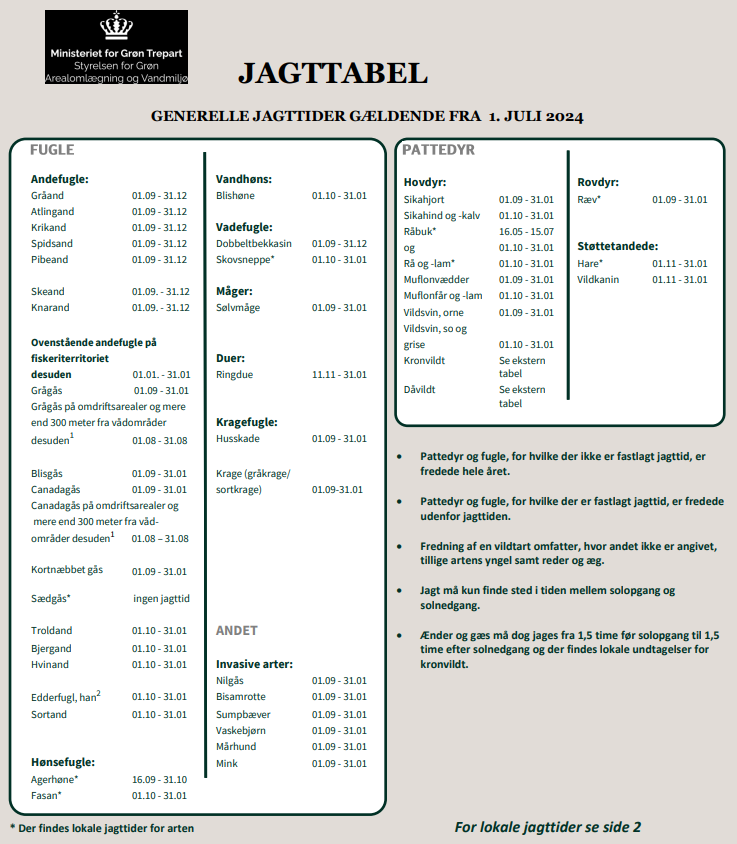
\includegraphics[width=0.42\textwidth]{Billeder/Andet/jagttider.png}
\end{frame}

\section{Vildtskadebekendtgørelsen}

\begin{frame}
  \vspace{3em}
  \begin{center}
    {\LARGE \textbf{Vildtskadebekendtgørelsen}}
    \vspace{2em}
    \\ Bekendtgørelse om vildtskader
\par
{\normalsize \href{https://www.retsinformation.dk/eli/lta/2026/708}{BEK nr 708 af 27/08/2026}}
\vspace{0.5em}
\par
{\small Senest opdateret: 4.\ september 2026}
\vspace{1em}
\par
  \end{center}
\end{frame}
\begin{frame}{Læringsmål ift. vildskadebekendtgørelsen}

\textbf{Vildtskader}

\vspace{0.2cm}

Jagttegnsaspiranter skal kende:

\begin{itemize}
    \item \textbf{Bekendtgørelse nr. 1408 af 3. oktober 2022 om vildtskader}
    \begin{itemize}
        \item (vildtskadebekendtgørelsen)
        \item Hele bekendtgørelsen
    \end{itemize}

    \item \textbf{Lov om jagt og vildtforvaltning}, senest bekendtgjort ved
    lovbekendtgørelse nr. 639 af 26. maj 2023
    \begin{itemize}
        \item (jagt- og vildtforvaltningsloven)
        \item §§ 37 og 38
    \end{itemize}
\end{itemize}

\vspace{0.2cm}

Loven og bekendtgørelsen omhandler reglerne for regulering af vildt.

\vspace{0.2cm}

I jagtprøven kan der stilles spørgsmål til konkrete arter, tidspunkter og
situationer, hvor man kan opnå tilladelse til regulering (ringdue, råge, grågås,
krage, husskade, ræv, mink, mårhund, vaskebjørn, husmår, ilder, vildsvin).

\end{frame}


\begin{frame}{Jagt og regulering}

\vspace{1em}

\small

\raggedright

\begin{itemize}

\itemsep0.6em % Justér afstand mellem bullets

\item \textbf{Regulering} er målrettet funktionel ned/ombringelse af specifik type vildt i et område, hvor \textbf{jagt} er rekreativ nedlæggelse af vildt med jagttider.

\item Formål: beskytte menneskers og dyrs sundhed, smitte, luffartssikkerhed, beskytte flora og fauna, skade på ejendom/landbrug mm.

\item Regulering er koblet til ejeren/brugeren af ejendom (kan ikke besluttes af andre).

\item Indehaver af reguleringstilladelse kan bemyndige person med jagttegn til at udføre reguleringen.

\end{itemize}

\end{frame}

\begin{frame}{Regulering uden foregående aftale (tilladelse)}

\vspace{1em}

\small

\raggedright

\begin{itemize}

\itemsep0.6em % Justér afstand mellem bullets

\item \textbf{Hjortevildt og hare} kan reguleres hele året i forsvarligt indhegnede områder med erhvervsmæssig drift til plateskole, gartneri og frugtplantager.

\item \textbf{Husmår og ilder} kan regulerers hele året i fjerkræsindhegninger, beboelse og pelsdyrfarme. Afstand til bebyggelse/hegn: (fælder indtil 10 m /skydevåben 25 m).

\item \textbf{Ræv} kan reguleres fra 1/6 - 29/2 ved indhegninger til fjerkræ og smågrise (bebyggelse/hegn: fælder indtil 10 m /skydevåben 25 m). Skade på øvrig fauna 1-29/2. Rævehvalpe må reguleres 1/7-31/8 udenfor rævegraven (men ikke i områder hvor der er gennemført naturforbedringer i henhold til biotopplaner). Kan skydes fra jagttårne og -stiger fra 1 time før til 1 time efter med glatløbet haglgevær og riflede våben. 

\item \textbf{Vildkanin} Kan reguleres hele året, såfremt den forvolder skade.

\end{itemize}

\end{frame}

\begin{frame}{Regulering uden foregående aftale (tilladelse) - \textit{fortsat}}

\vspace{1em}

\small

\raggedright

\begin{itemize}

\itemsep0.6em % Justér afstand mellem bullets

\item \textbf{Vildsvin} kan reguleres hele året. Kan reguleres hele døgnet. Må skydes på foderpladsen med kunstigt lys etc. 

\item \textbf{Særlige arter} Invasive arter fastsættes af EU. Omfatter bl.a nilgås, bisamrotte, sikavildt, amerikansk skarveand, muntjak, mårhund m.fl.     


\end{itemize}

\end{frame}

\begin{frame}{Regulering efter forudgående tilladelse}

\vspace{1em}

\small

\raggedright

\begin{itemize}
\itemsep0.6em


\item \textbf{Råge (§ 12)}: Tilladelse til regulering i flokke på marker (1. juli–30. sept.), i kolonier før æglægning (15. jan.–15. marts), unger uden for rede (1. maj–15. juni), unger på marker (1. maj–30. juni) samt hele året i gartnerier/frugtplantager mv.

\end{itemize}

\end{frame}

\begin{frame}{Regulering efter forudgående tilladelse - \textit{fortsat}}

\vspace{1em}

\small

\raggedright

\begin{itemize}
\itemsep0.6em

\item \textbf{Husskade (§ 16)}: Regulering hvor skade på afgrøder eller fauna (1. feb.–15. april) med skydevåben/fælder, fra 1 time før solopgang til solnedgang (fælder hele døgnet). Mulighed for kunstigt skjul og lokkefugle.

\item \textbf{Gråkrage og sortkrage (§ 17)}: Som husskade – regulering ved skade på afgrøder/fauna (1. feb.–15. april), samt hele året i gartnerier/frugtplantager mv. Mulighed for kunstigt skjul og lokkefugle.

\item \textbf{Ringdue (§ 18)}: Regulering i flokke på raps (feb.–apr.), ærter/kål/nysåede marker (marts–apr. + aug.), ikke høstede marker (juli–aug.). Ved omfattende skade sep.–10. nov. Hele året i gartnerier mv.

\end{itemize}

\end{frame}

\begin{frame}{Regulering efter forudgående tilladelse - \textit{fortsat 2}}

\vspace{1em}

\small

\raggedright

\begin{itemize}
\itemsep0.6em

\item \textbf{Grågås (§ 19)}: Regulering i flokke på ikke høstede marker (juli) og dyrkede marker (feb.), fra solopgang til solnedgang.

\item \textbf{Ræv (§ 26)}: Regulering i indhegninger med fårehold (læmningsperiode), frilandsgrise/fjerkræ/fasaner mv. (marts–maj), samt nær indhegninger og bebyggelse med fælder/skydevåben.

\end{itemize}

\end{frame}

\begin{frame}{Regulering efter forudgående tilladelse - \textit{fortsat 3}}

\vspace{1em}

\small

\raggedright

\begin{itemize}
\itemsep0.6em

\item \textbf{Arter (§ 27)}: Undslupne pelsdyr (vildt ifølge mark- og vejfredsloven), mårhund, mink, vaskebjørn, sumpbæver og bisamrotte.

\item Naturstyrelsen kan give tilladelse til regulering fra 1 time efter solnedgang til 1 time før solopgang.

\item Tilladelse inkluderer: Regulering fra kunstigt skjul (inkl. skydestiger og -tårne).

\item Tilladelse inkluderer: Brug af kunstigt lys, spejle og andre indretninger til belysning af målet (uanset forbud i udsætningsbekendtgørelsen).

\end{itemize}

\end{frame}

\begin{frame}{Regulering efter forudgående tilladelse - \textit{fortsat 4}}

\vspace{1em}

\small

\raggedright

\begin{itemize}
\itemsep0.6em

\item Reguleringen skal udføres i overensstemmelse med § 1, stk. 2, i bekendtgørelse om udsætning af vildt, jagtmåder og jagtredskaber.

\item \textbf{Stk. 2}: Tilladelse til udfodring og beskydning på jorden i umiddelbar nærhed af foderplads.

\item \textbf{Stk. 3}: Tilladelse til anvendelse af motordrevet køretøj ved regulering af arterne i stk. 1 samt mårhund og vaskebjørn (efter § 8).

\end{itemize}

\end{frame}

\begin{frame}{Brug af fælder - Generelle krav (§ 34)}

\vspace{1em}

\small

\raggedright

\begin{itemize}
\itemsep0.6em

\item Fælder skal indrettes så fangne dyr ikke skades eller dræbes.

\item Fangne dyr må ikke komme i fysisk kontakt med hinanden.

\item Fangne dyr skal kunne besigtiges i fælden, når denne er lukket.

\item Fælden må anvendes hele døgnet og skal efterses hver dag morgen og aften (jf. dog § 36 stk. 2).

\item Ved eftersyn: Fangne dyr udtages straks. Forbudte dyr frigives straks (jf. dog § 35). Øvrige ombringes i eller umiddelbart efter udtagelse (uanset § 23 i jagt- og vildtforvaltningsloven).

\end{itemize}

\end{frame}

\begin{frame}{Brug af fælder - Generelle krav (§ 34) - \textit{fortsat}}

\vspace{1em}

\small

\raggedright

\begin{itemize}
\itemsep0.6em

\item Fælden må ikke nedgraves.

\item Fælden skal være tydeligt mærket med ansvarliges kontaktoplysninger og formål.

\item Fælden skal deaktiveres i perioder/steder, hvor fangst ikke er tilladt.

\item Fælden skal være flytbar og en fast konstruktion.

\end{itemize}

\vspace{1em}

\end{frame}

\begin{frame}{Brug af fælder til pattedyr (§ 35)}

\begin{columns}[T]  % T = top-aligned (så teksten starter øverst ligesom billedet)

\begin{column}{0.58\textwidth}  % venstre kolonne – ca. 58% til tekst (juster efter behov)
\vspace{1em}
\small
\raggedright

\begin{itemize}
\itemsep0.6em

\item Fangstrum max 60 (H) × 60 (B) × 250 (L) cm.

\item Indgangsåbninger placeret i enden af fælden.

\item For ræv og mårhund: Indgang max 60 × 60 cm. For andre pattedyr (mink/husmår): Max 60 × 60 cm.

\item Ved bifangst af arter fra § 8 i fælde med indgang 30–60 cm: Frigivelseskrav gælder ikke.

\item Fælder skal være overdækkede (lokkemad kun synlig gennem enderne).

\end{itemize}

\end{column}

\begin{column}{0.40\textwidth}  % højre kolonne – ca. 40% til billede (juster 0.58 + 0.40 ≈ 0.98 for at undgå overflow)
\centering
\vspace{0.5em}  % lille top-margin så billedet ikke klistrer helt op

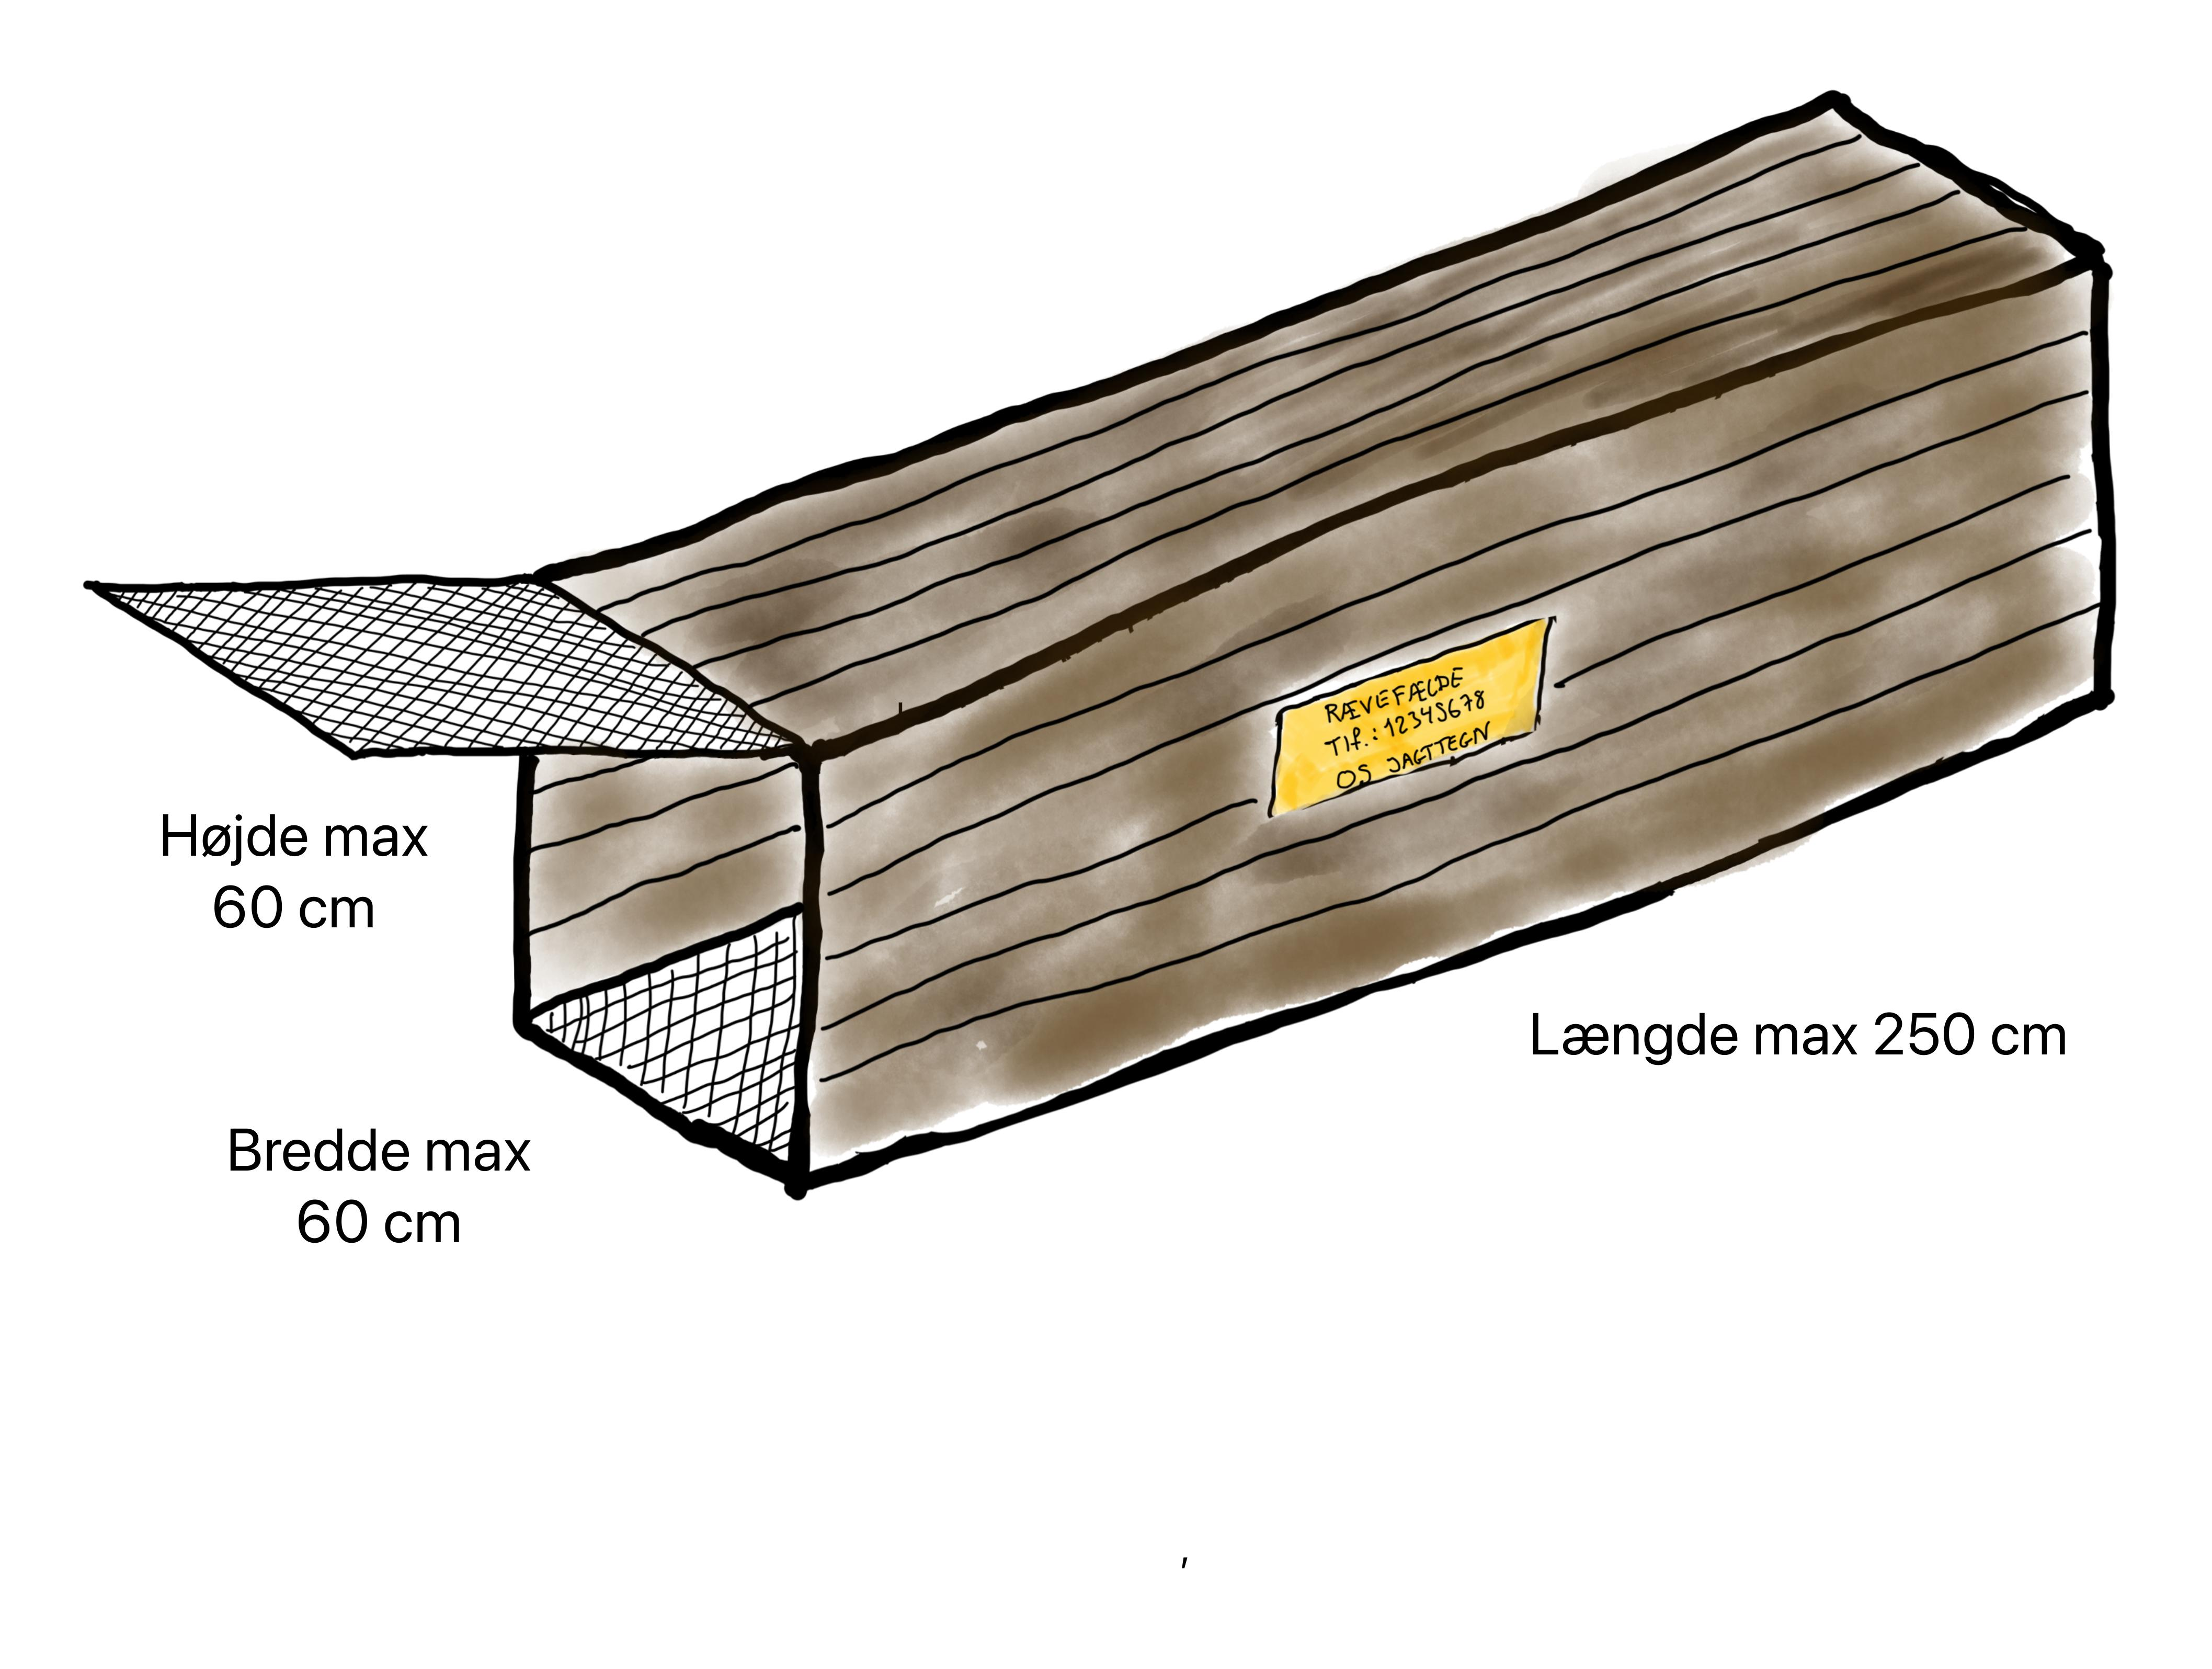
\includegraphics[width=\textwidth,height=0.75\textheight,keepaspectratio]{Billeder/Redskaber/raevefaelde.jpg}
% eller: [width=0.9\textwidth] hvis du vil have det lidt mindre

% Alternativt med figur-caption hvis du vil:
% \begin{figure}
%   \includegraphics[width=\textwidth]{dit_billede.jpg}
%   \caption{Eksempel på en rævefælde}
% \end{figure}

\end{column}

\end{columns}

\end{frame}

\begin{frame}{Brug af fælder til fugle (skrå sider)}

\begin{columns}[T]  % Top-aligned så tekst og billede starter i samme højde

\begin{column}{0.58\textwidth}  % Venstre: tekst (ca. 58 % bredde)
\vspace{1em}
\small
\raggedright

\begin{itemize}
\itemsep0.6em

\item Fangstrum max 60 (H) × 60 (B) × 250 (L) cm.

\item Indgangsåbninger ovenpå eller skråtstillet (40–50 grader). Ovenpå: Max 40 × 40 cm. Skrå: Max 60 × 40 cm.

\item Må ikke bruge kød eller ådsler som lokkemad.

\item Eftersyn morgen/aften kan erstattes af elektronisk enhed (f.eks. SMS-sender): Max 12 timer til fysisk tilsyn efter udløsning eller fejl. Fysisk tilsyn min. 1× dagligt første 3 dage.

\end{itemize}

\end{column}

\begin{column}{0.40\textwidth}  % Højre: billede (ca. 40 % bredde)
\centering
\vspace{0.5em}  % Lille top-margin for bedre balance

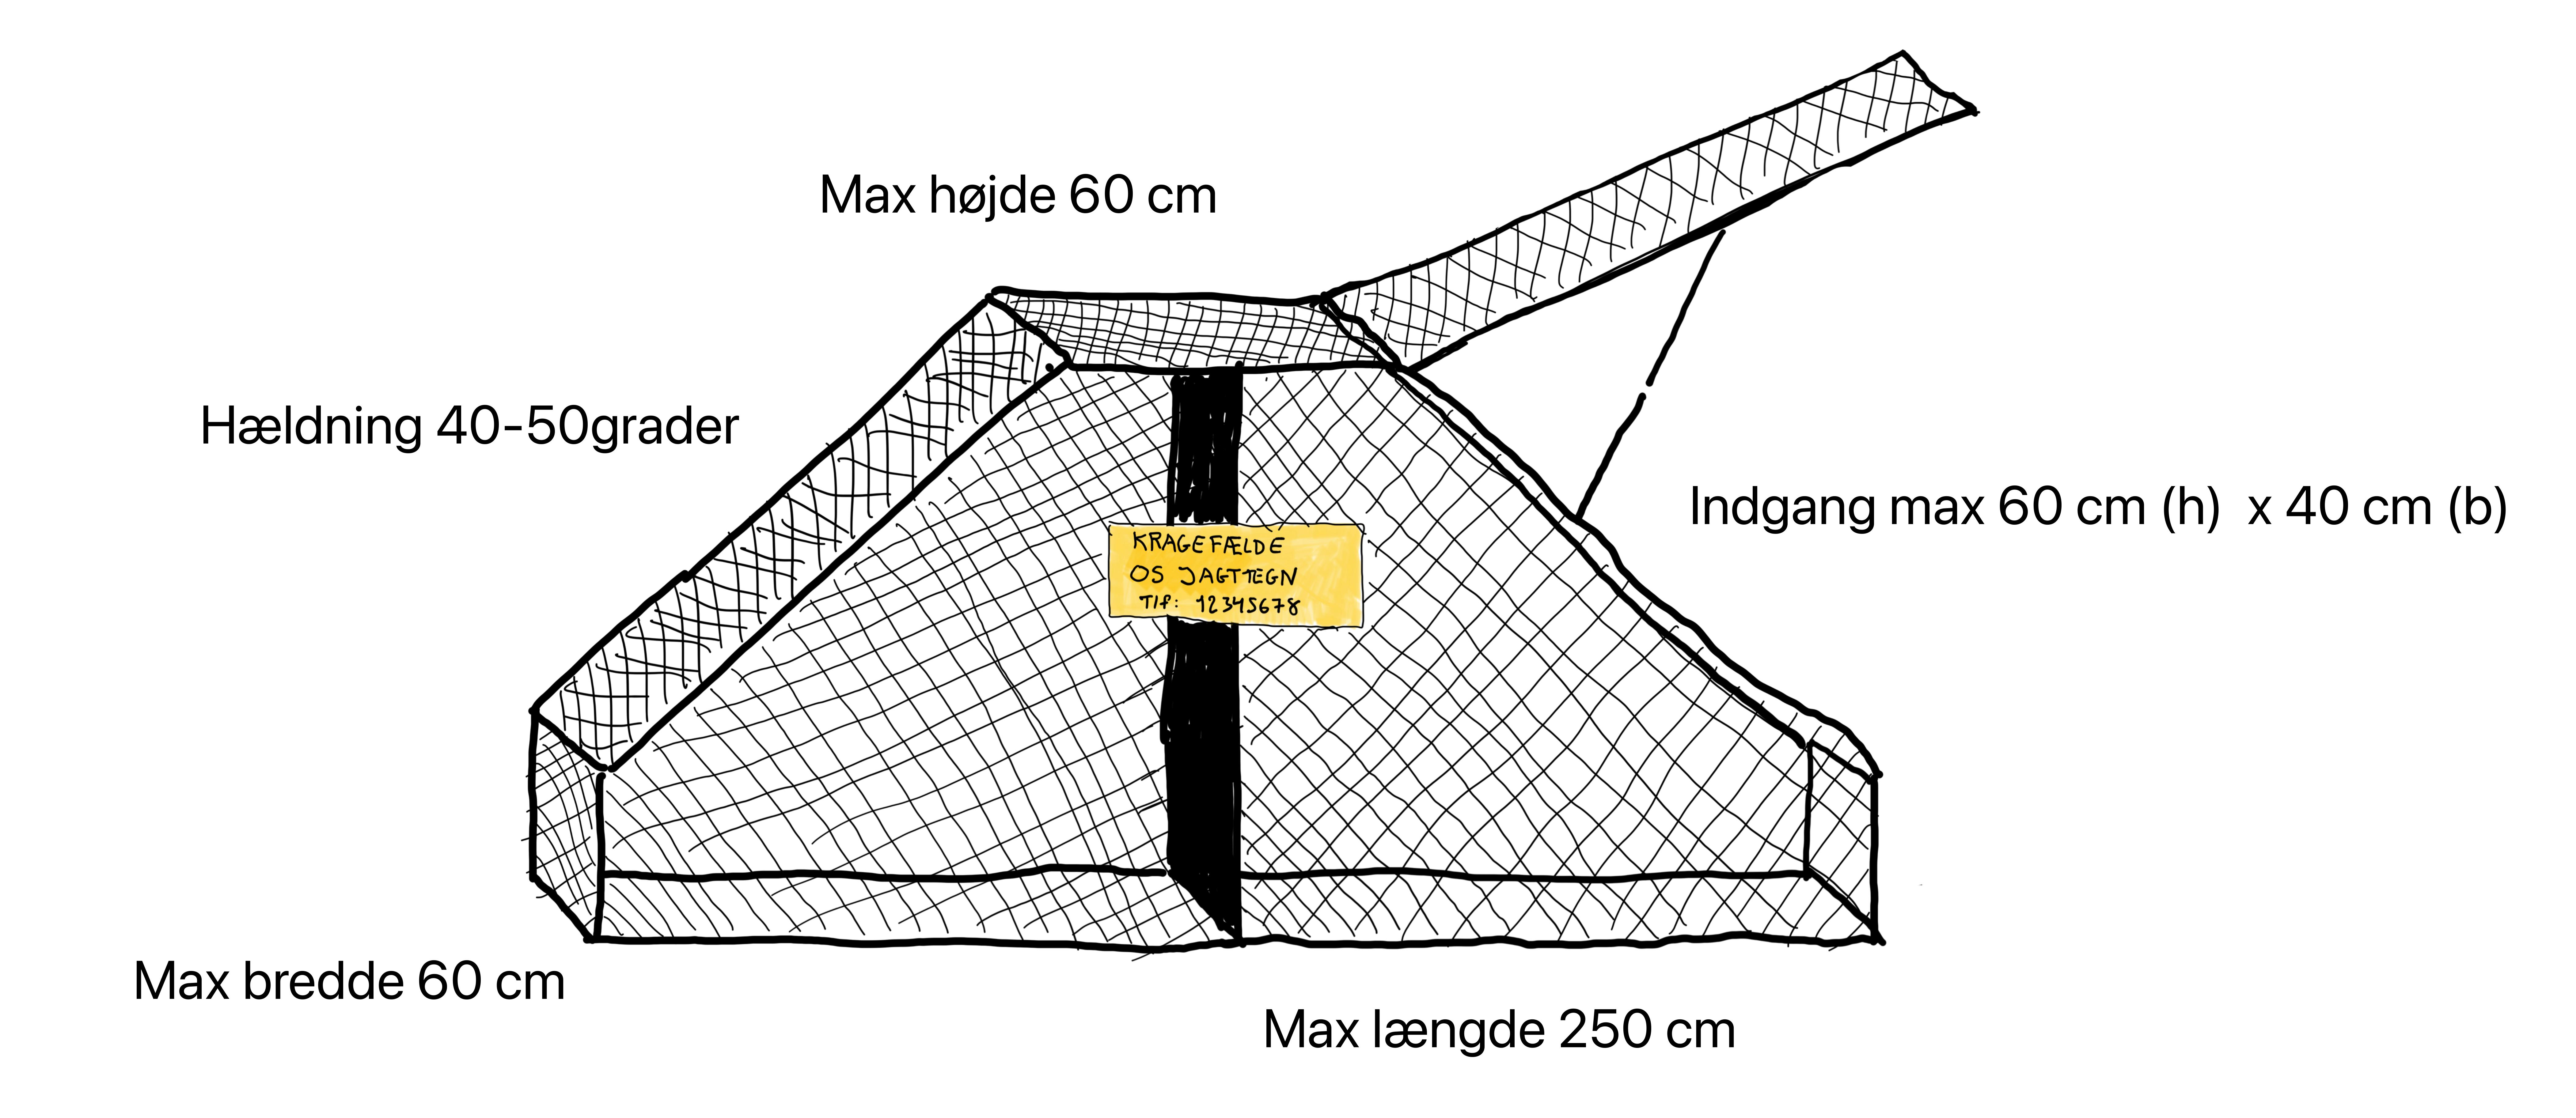
\includegraphics[width=\textwidth,height=0.75\textheight,keepaspectratio]{Billeder/Redskaber/fuglefaelde_skraa.jpg}
% Alternativer du kan prøve:
% \includegraphics[width=0.95\textwidth]{dit_billede.jpg}          % Lidt luft rundt om
% \includegraphics[height=0.7\textheight,keepaspectratio]{...}     % Begræns højde hvis billedet er højt

% Hvis du vil have en lille caption under billedet:
% \vspace{0.5em}
% \tiny Eksempel på fælde med skrå indgang (kilde: Naturstyrelsen eller lign.)

\end{column}

\end{columns}

\end{frame}

\begin{frame}{Brug af fælder til fugle (lige sider)}

\begin{center}
\vspace{0.5em}  % Lille top-margin for bedre balance på slide

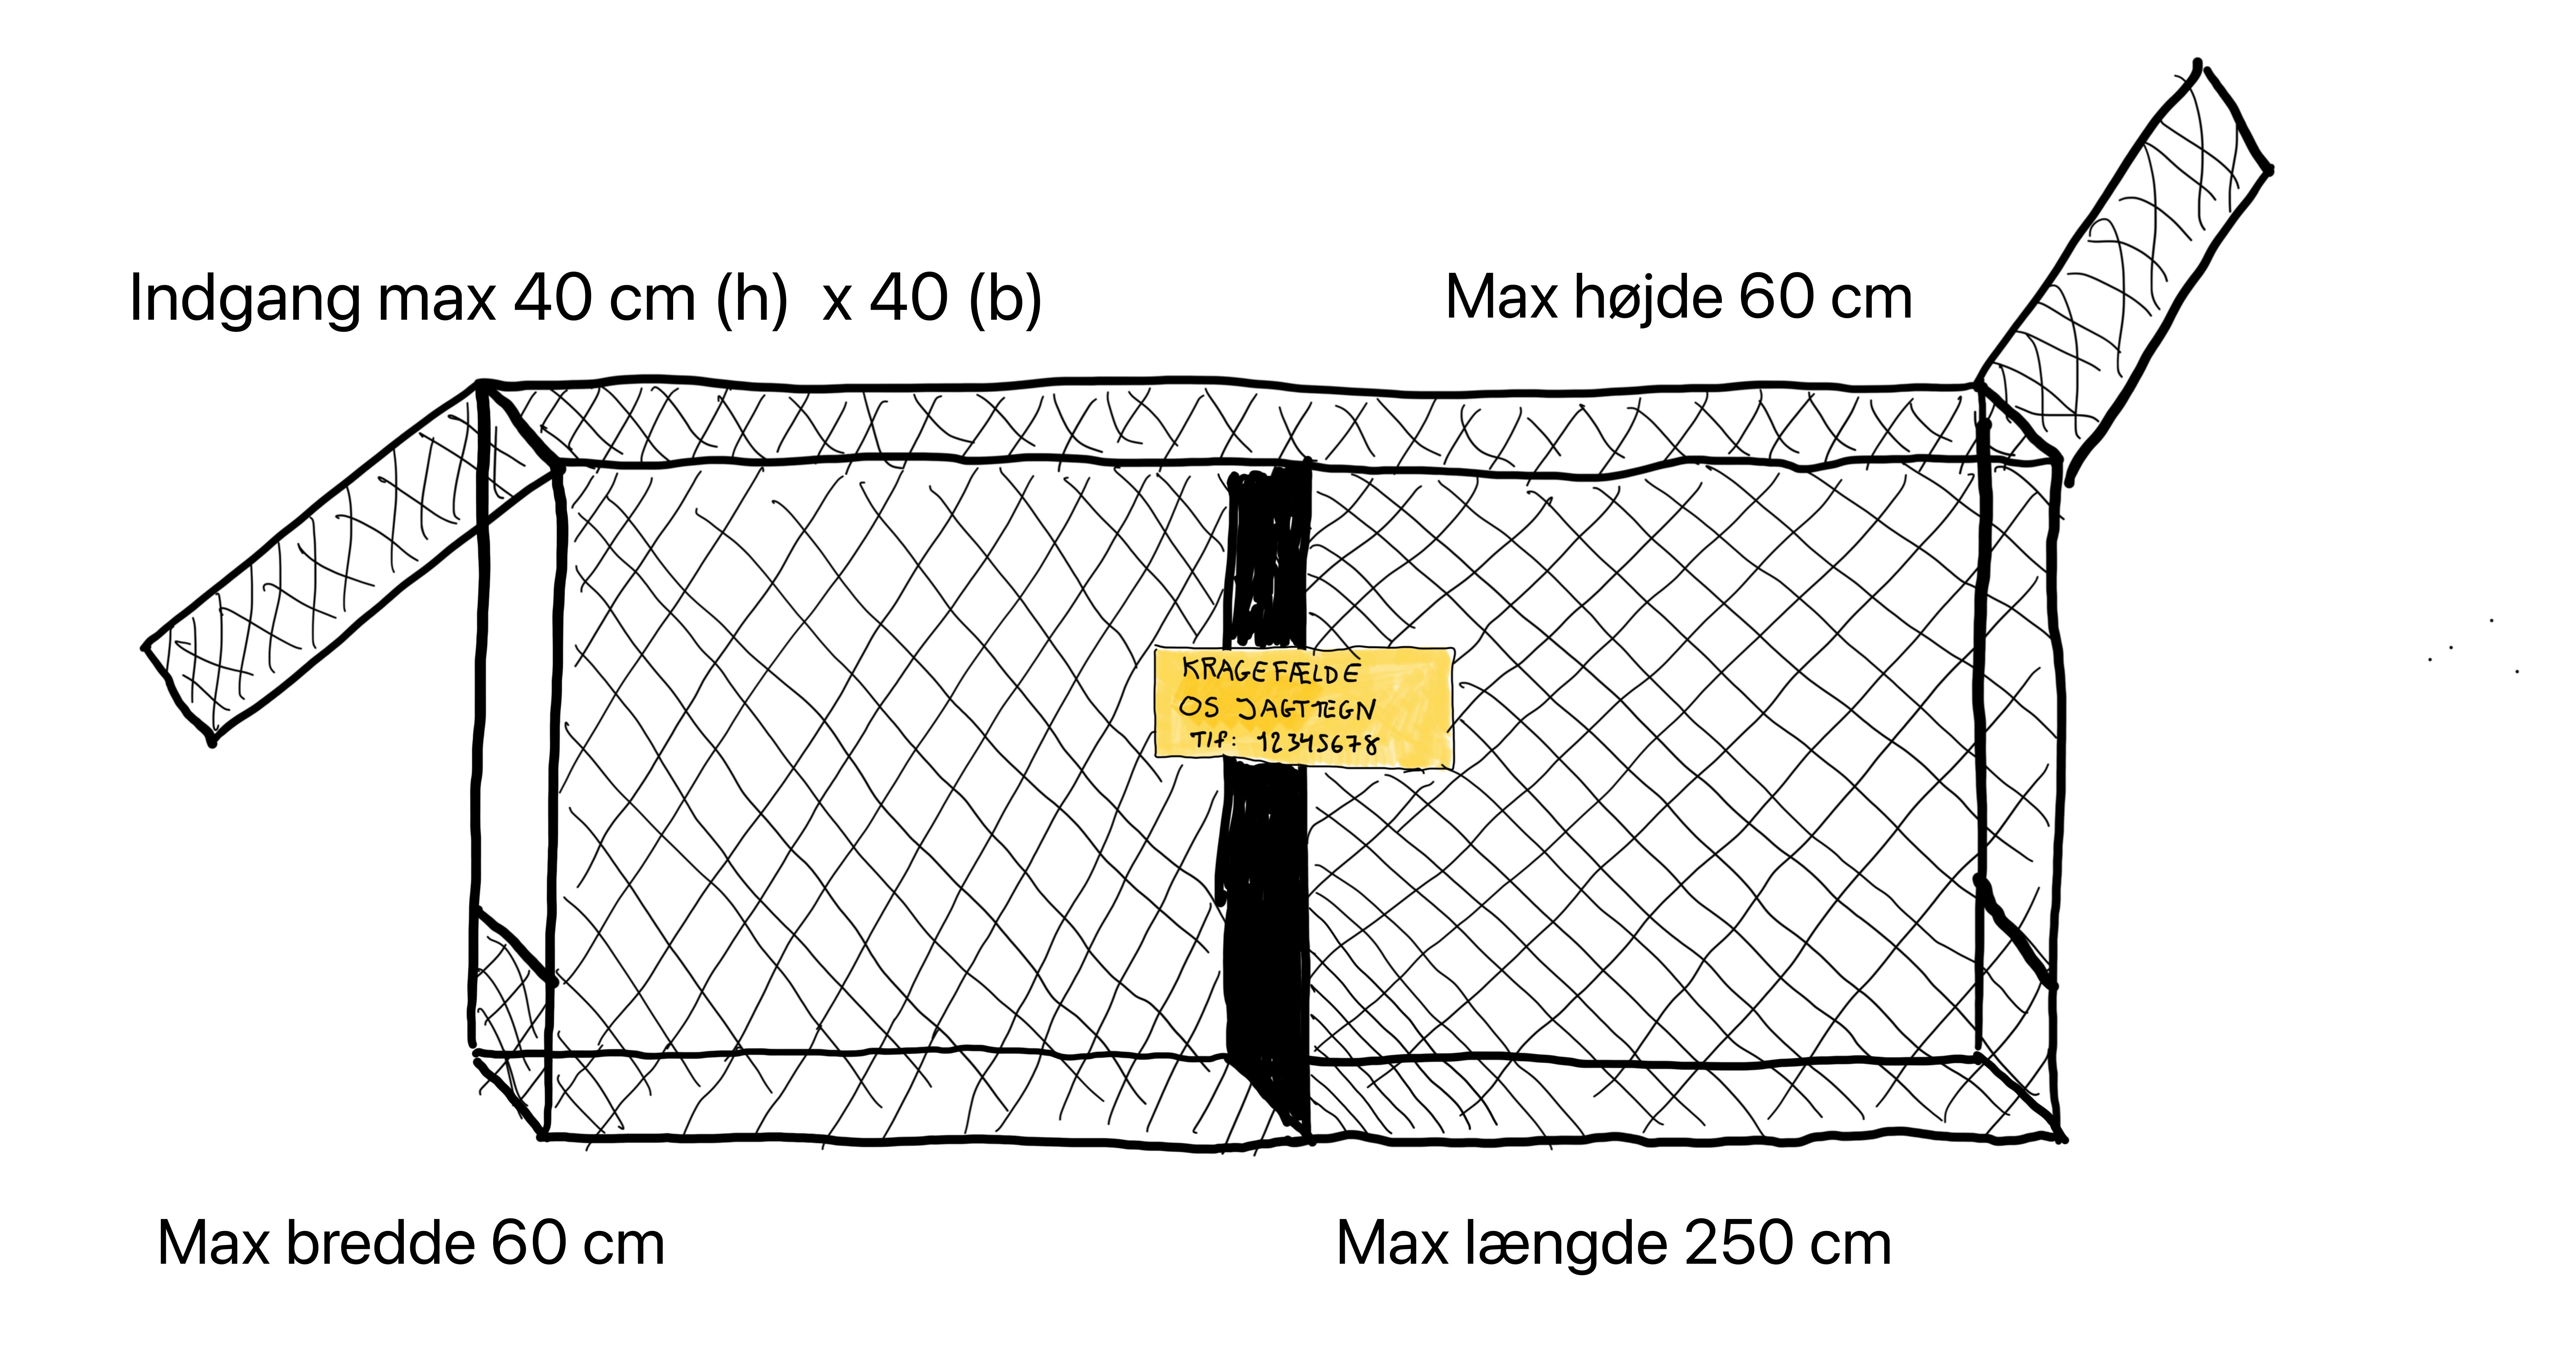
\includegraphics[height=0.85\textheight,keepaspectratio]{Billeder/Redskaber/fuglefaelde_lige.jpg}
% Alternativer du kan prøve for bedre pasform:
% \includegraphics[width=0.95\textwidth,keepaspectratio]{dit_billede.jpg}  % Bredde-prioriteret
% \includegraphics[width=\textwidth,height=0.8\textheight,keepaspectratio]{...}

% Valgfri lille caption under billedet (hvis du vil have det):
% \vspace{0.5em}
% \tiny Eksempel på fælde med skrå eller ovenpå-indgang (40–50 grader)

\end{center}

\end{frame}

\section{Svømmeænder}

\begin{frame}
  \vspace{3em}
  \begin{center}
    {\LARGE \textbf{Svømmeænder}}
    \vspace{2em}
    \\ Artsbestemmelse og vildtbiologi
\par
% Våbenbekendtgørelsen
{\normalsize }
\vspace{1em}
\par
  \end{center}
\end{frame}


\begin{frame}{Artsbiologi: tre vidensniveauer}
  \vspace{0.8em}
 
  \centering
  \small
  \begin{tabular}{l|c|c|c}
    \toprule
    % STARTE MED IKONERNE
    % Bruger nu dit eget billede i stedet for \star
    & \textbf{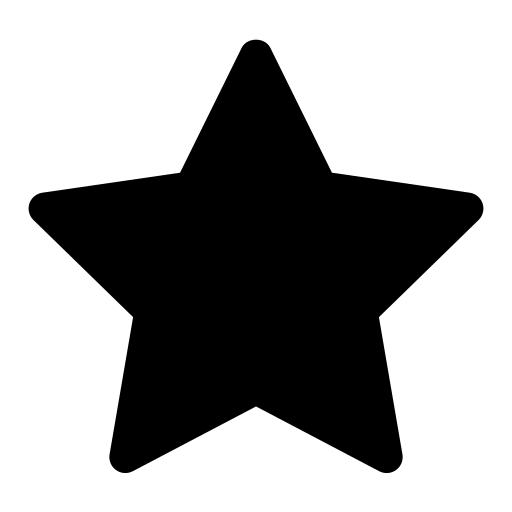
\includegraphics[width=0.4cm]{Billeder/Ikoner/star_black.png}} 
    & \textbf{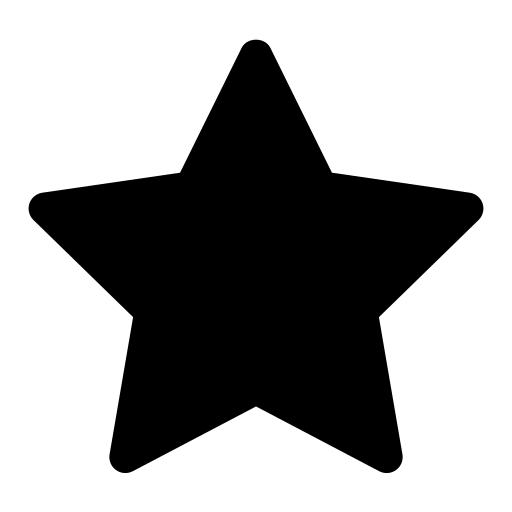
\includegraphics[width=0.4cm]{Billeder/Ikoner/star_black.png}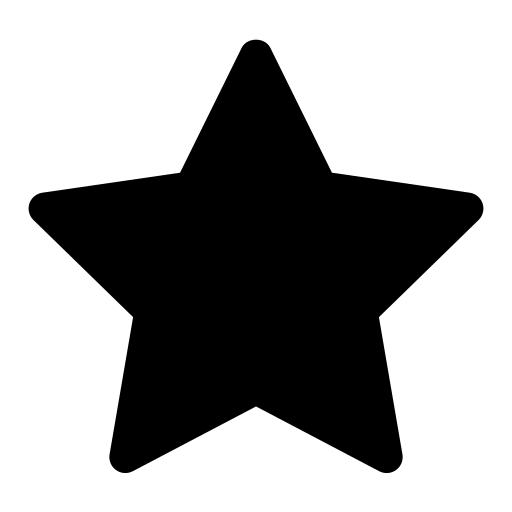
\includegraphics[width=0.4cm]{Billeder/Ikoner/star_black.png}} 
    & \textbf{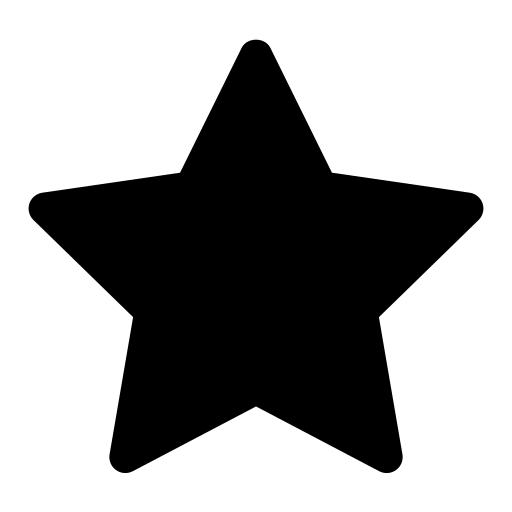
\includegraphics[width=0.4cm]{Billeder/Ikoner/star_black.png}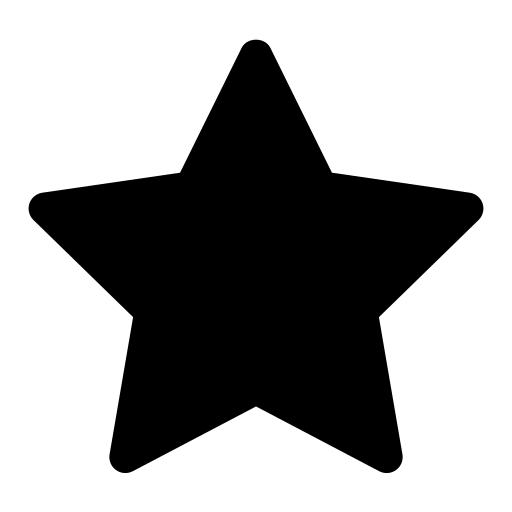
\includegraphics[width=0.4cm]{Billeder/Ikoner/star_black.png}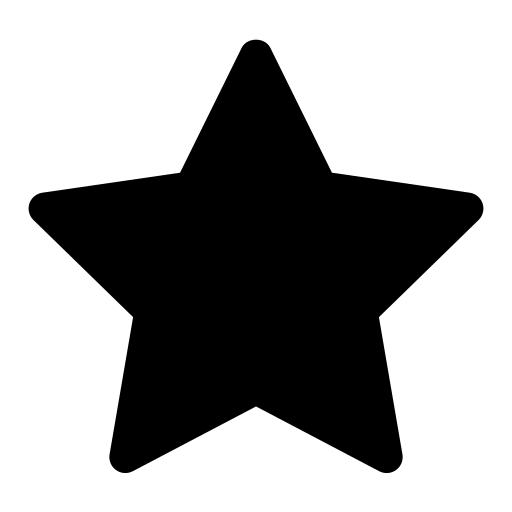
\includegraphics[width=0.4cm]{Billeder/Ikoner/star_black.png}} \\
    \midrule % <-- STREG: Adskiller ikoner fra tekstoverskrifter
    % DEREFTER TEKSTOVERSKRIFTERNE
    & \textbf{Genkendelse} & \textbf{Basal biologi} & \textbf{Udvidet biologi} \\
    \midrule % <-- STREG: Adskiller overskrifter fra data
    \textbf{Udseende} & $\checkmark$ & $\checkmark$ & $\checkmark$ \\
    \textbf{Levesteder} & & $\checkmark$ & $\checkmark$ \\
    \textbf{Føde} & & $\checkmark$ & $\checkmark$ \\
    \textbf{Udbredelse} & & $\checkmark$ & $\checkmark$ \\
    \textbf{Træk/standfugl} & & $\checkmark$ & $\checkmark$ \\
    \textbf{Yngleforhold} & & & $\checkmark$ \\
    \textbf{Kønsmoden} & & & $\checkmark$ \\
    \textbf{Mono/polygam} & & & $\checkmark$ \\
    \textbf{Bestandsomsætning} & & & $\checkmark$ \\
    \textbf{Kuld størrelse} & & & $\checkmark$ \\
    \bottomrule
  \end{tabular}
\end{frame}

\begin{frame}{Svømmeænder vs Dykænder}
  \vspace{1.5em}
  \centering
  \small
  \begin{tabular}{@{}p{0.45\textwidth}|p{0.45\textwidth}@{}}
    \textbf{Svømmeænder} & \textbf{Dykænder} \\
    \hline
    Spiser ved overfladen & Spiser ved sø/havbunden \\[0.4em]
    Fødder midt på kroppen & Fødder bag på kroppen \\[0.4em]
    Store vinger – adræt i luften & Små vinger – adræt under vandoverfladen \\[0.4em]
    Trives på lavere vand & Trives på dybere vand \\
  \end{tabular}
\end{frame}

% ========== GRÅAND ==========
\begin{frame}{%
  \begin{minipage}[t]{0.32\textwidth}
    Gråand
  \end{minipage}%
  \hfill
  \begin{minipage}[t]{0.36\textwidth}
    \centering
    \footnotesize\textbf{Jagttid:} 1.\ september -- 31.\ januar
  \end{minipage}%
  \hfill
  \begin{minipage}[t]{0.15\textwidth}
    \noindent\raggedleft
    
\includegraphics[width=0.5cm, height=0.5cm, keepaspectratio]{Billeder/Ikoner/star.png}%
    \hspace{0.2em}%
    
\includegraphics[width=0.5cm, height=0.5cm, keepaspectratio]{Billeder/Ikoner/star.png}%
    \hspace{0.2em}%
    
\includegraphics[width=0.5cm, height=0.5cm, keepaspectratio]{Billeder/Ikoner/star.png}
  \end{minipage}%
}
  \vspace{0.25em}
  \begin{columns}[T]
    % --- Venstre kolonne: Tekst ---
    \column{0.55\textwidth}
    \setlength{\parskip}{0.5em}
    \tiny
    \RaggedRight
    \textbf{\textit{Anas platyrhynchos}} – stor svømmeand med rappende kald, også kaldet vildand, moseand, stokand \par
    \textbf{Udseende:}\\
    \quad – Andrik: Hvid halsring, metalblåt vingespejl \par
    \quad – And: Gulligt næb, blåt vingespejl \par
    \textbf{Levesteder:} Søer, moser, fjorde og vandløb. \par
    \textbf{Føde:} Dyre- og planteføde, herunder hvede og byg. \par
    \textbf{Udbredelse:} Hele Danmark. \par
    \textbf{Træk/standfugl:} Begge (trækfuglene kommer efter oktober)
    \begin{itemize}
      \itemsep0pt
      \item \textbf{Yngleforhold:} Yngler i hele Danmark.
      \item \textbf{Kønsmoden:} Ca. 1 år
      \item \textbf{Mono/polygam:} Monogam
      \item \textbf{Bestandsomsætning:} Hurtig
      \item \textbf{Kuld:} 9–13 æg
      \item \textbf{Jagttid:} 1.\ september -- 31.\ januar
    \end{itemize}
    % --- Højre kolonne: Billeder ---
    \column{0.40\textwidth}
    \centering
    \fbox{%
      \begin{minipage}{\linewidth}
        \centering
        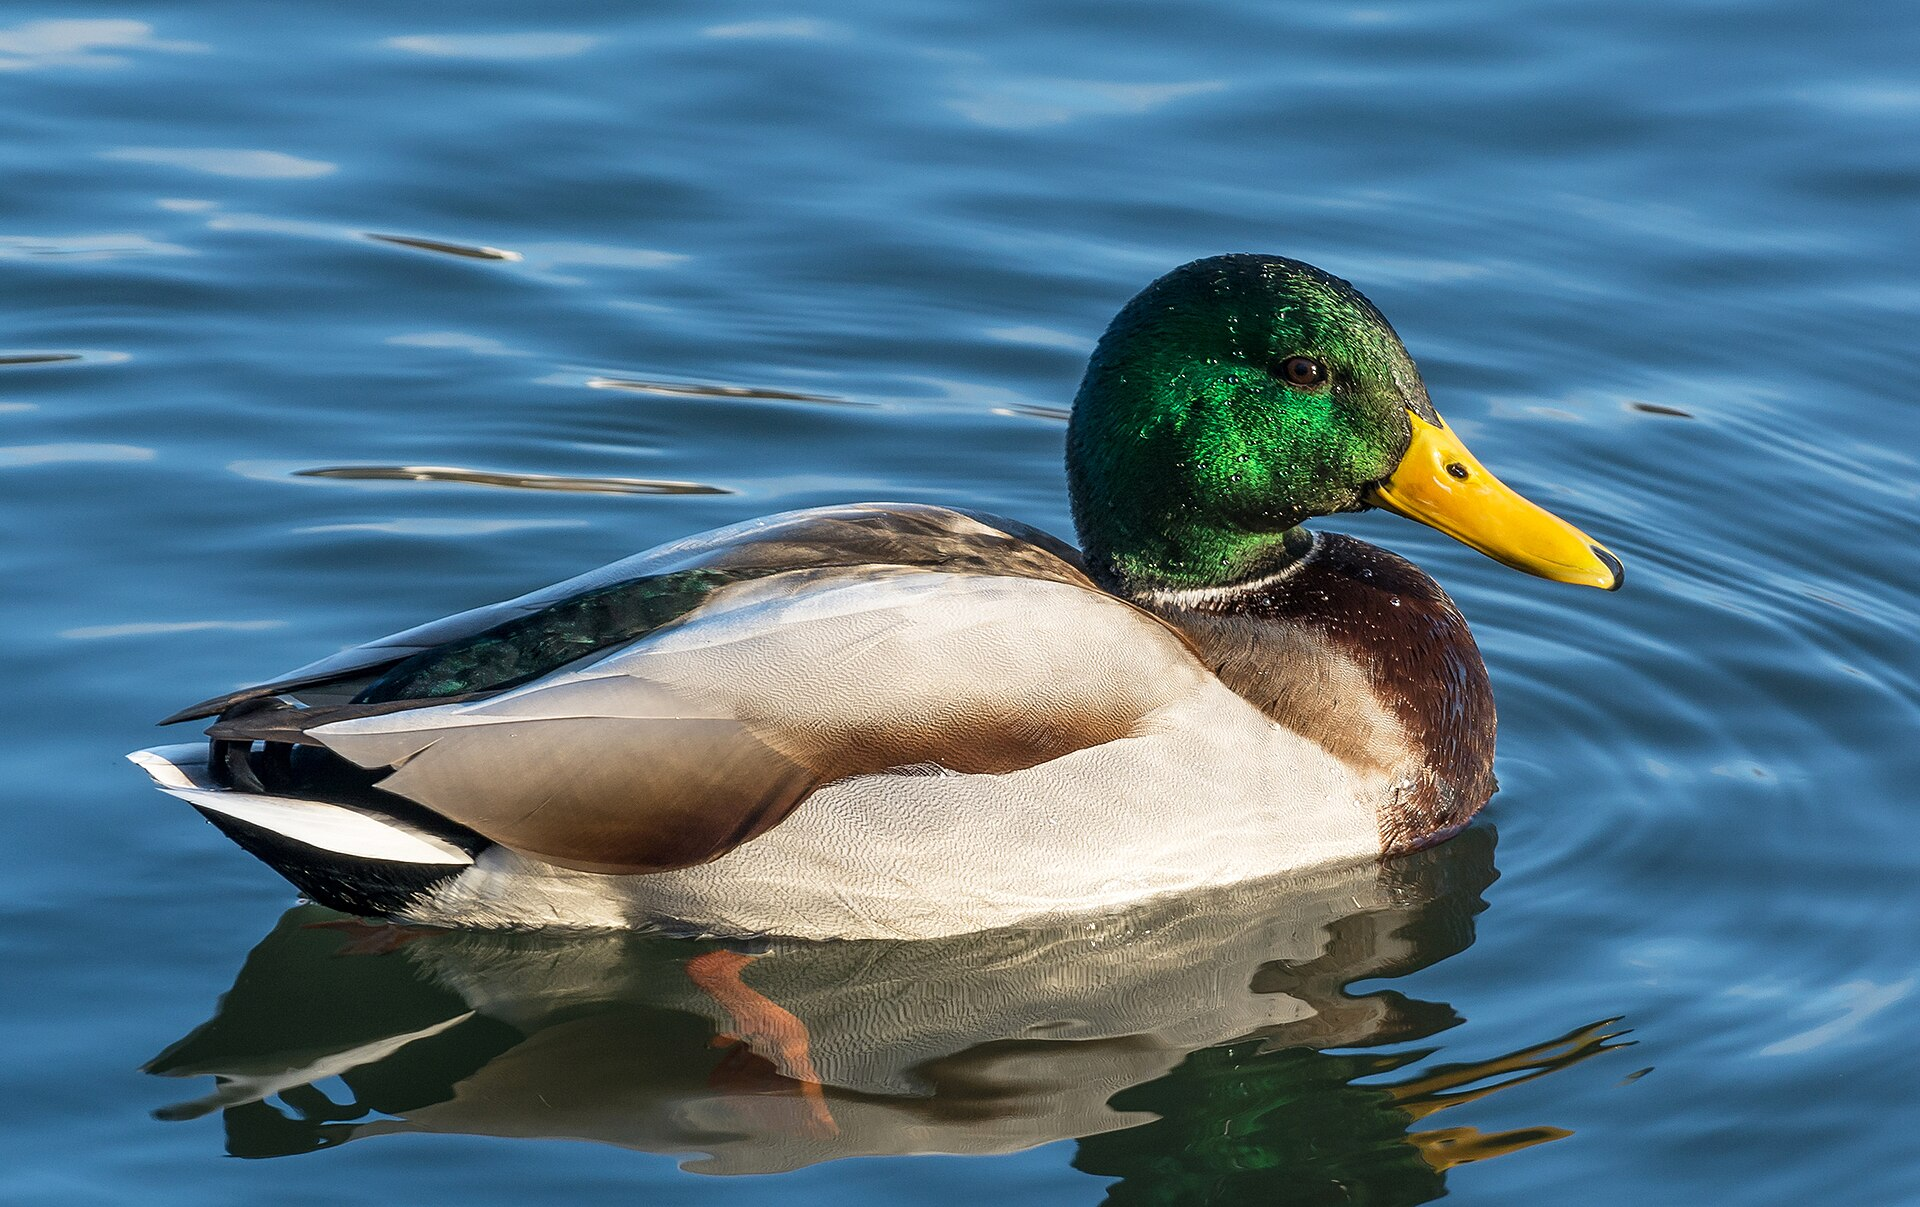
\includegraphics[width=0.7\linewidth, height=3cm, keepaspectratio]{Billeder/Dyr/Fugle/Aender/Svoemmeaender/gråand_han.jpg}\\[0.5em]
        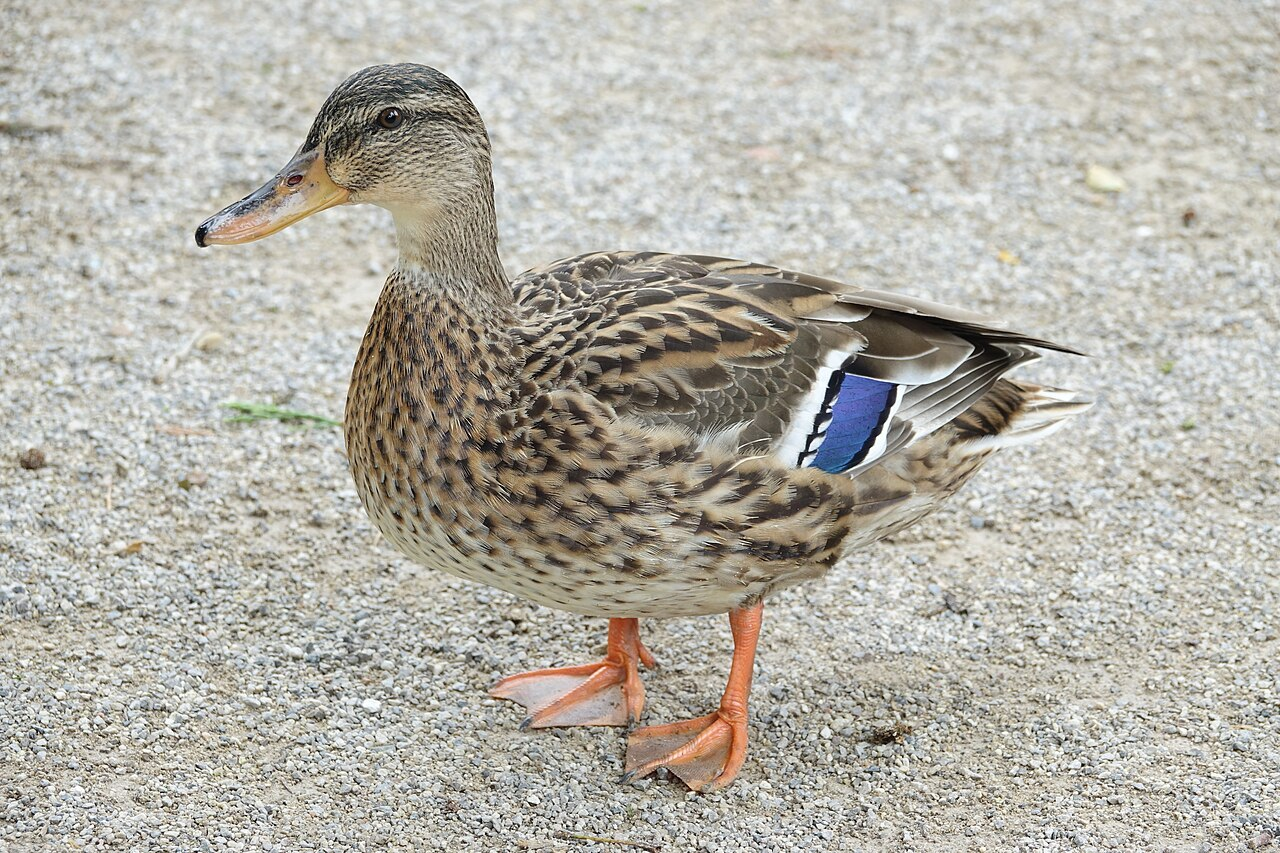
\includegraphics[width=0.7\linewidth, height=3cm, keepaspectratio]{Billeder/Dyr/Fugle/Aender/Svoemmeaender/gråand_hun.jpg}%
      \end{minipage}
    }%
    \vspace{0.05em}
    \footnotesize Andrik øverst, and nederst
  \end{columns}
\end{frame}
% Pibeand
\begin{frame}{%
  \begin{minipage}[t]{0.32\textwidth}
    Pibeand
  \end{minipage}%
  \hfill
  \begin{minipage}[t]{0.36\textwidth}
    \centering
    \footnotesize\textbf{Jagttid:} 1.\ september -- 31.\ december
  \end{minipage}%
  \hfill
  \begin{minipage}[t]{0.15\textwidth}
    \noindent\raggedleft
    
\includegraphics[width=0.5cm, height=0.5cm, keepaspectratio]{Billeder/Ikoner/star.png}%
    \hspace{0.2em}%
    
\includegraphics[width=0.5cm, height=0.5cm, keepaspectratio]{Billeder/Ikoner/star.png}
  \end{minipage}%
} % Ændret: Højre minipage nu med begge ikoner side om side
  \vspace{0.25em}
  \begin{columns}[T]
    % --- Venstre kolonne: Tekst ---
    \column{0.55\textwidth}
    \setlength{\parskip}{0.5em}
    \small
    \RaggedRight\textbf{\textit{Anas penelope}} – mellemstor svømmeand med pibende fløjt, også kaldet brunnakke \par

    \textbf{Udseende:} \\
    \quad – Andrik: rødbrunt hoved, blå-grønt næb, hvide skuldre \\
    \quad – And: blå-grønt næb \par

    \textbf{Levesteder:} \\
    \quad – Kystnære engarealer

    \textbf{Føde:} \\
    \quad – Plantearter, kogleaks \par

    \textbf{Udbredelse:} \\
    \quad – Hele Danmark \par

    \textbf{Træk/standfugl} \\
    \quad – Primært trækfugl \par

    % --- Højre kolonne: To billeder stablet over hinanden (større størrelse) ---
    \column{0.40\textwidth}
    \centering
    \fbox{%
      \begin{minipage}{\linewidth}
        \centering
        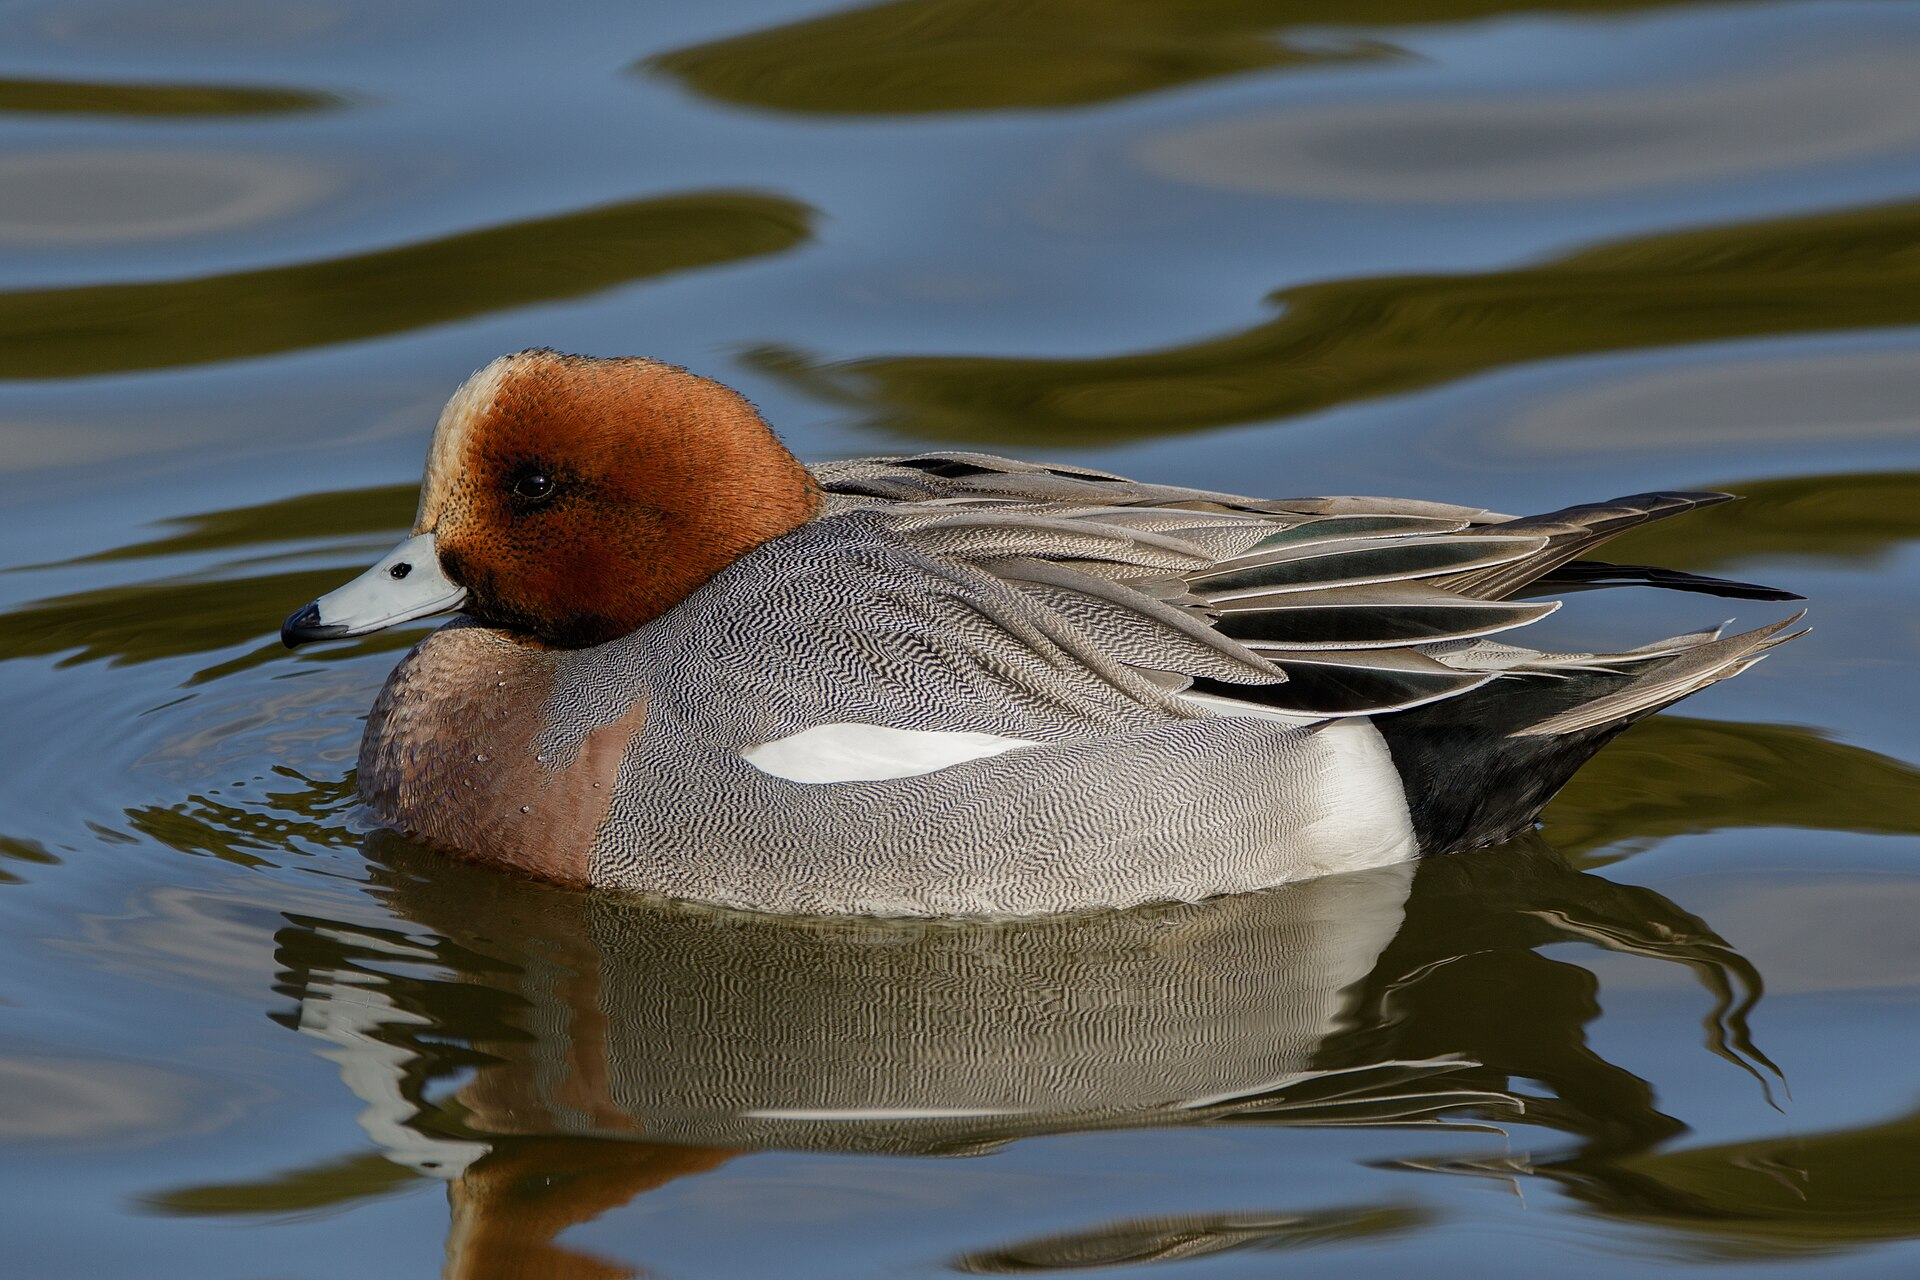
\includegraphics[width=0.8\linewidth, height=3.5cm, keepaspectratio]{Billeder/Dyr/Fugle/Aender/Svoemmeaender/pibeand_han.jpg}\\[0.5em]
        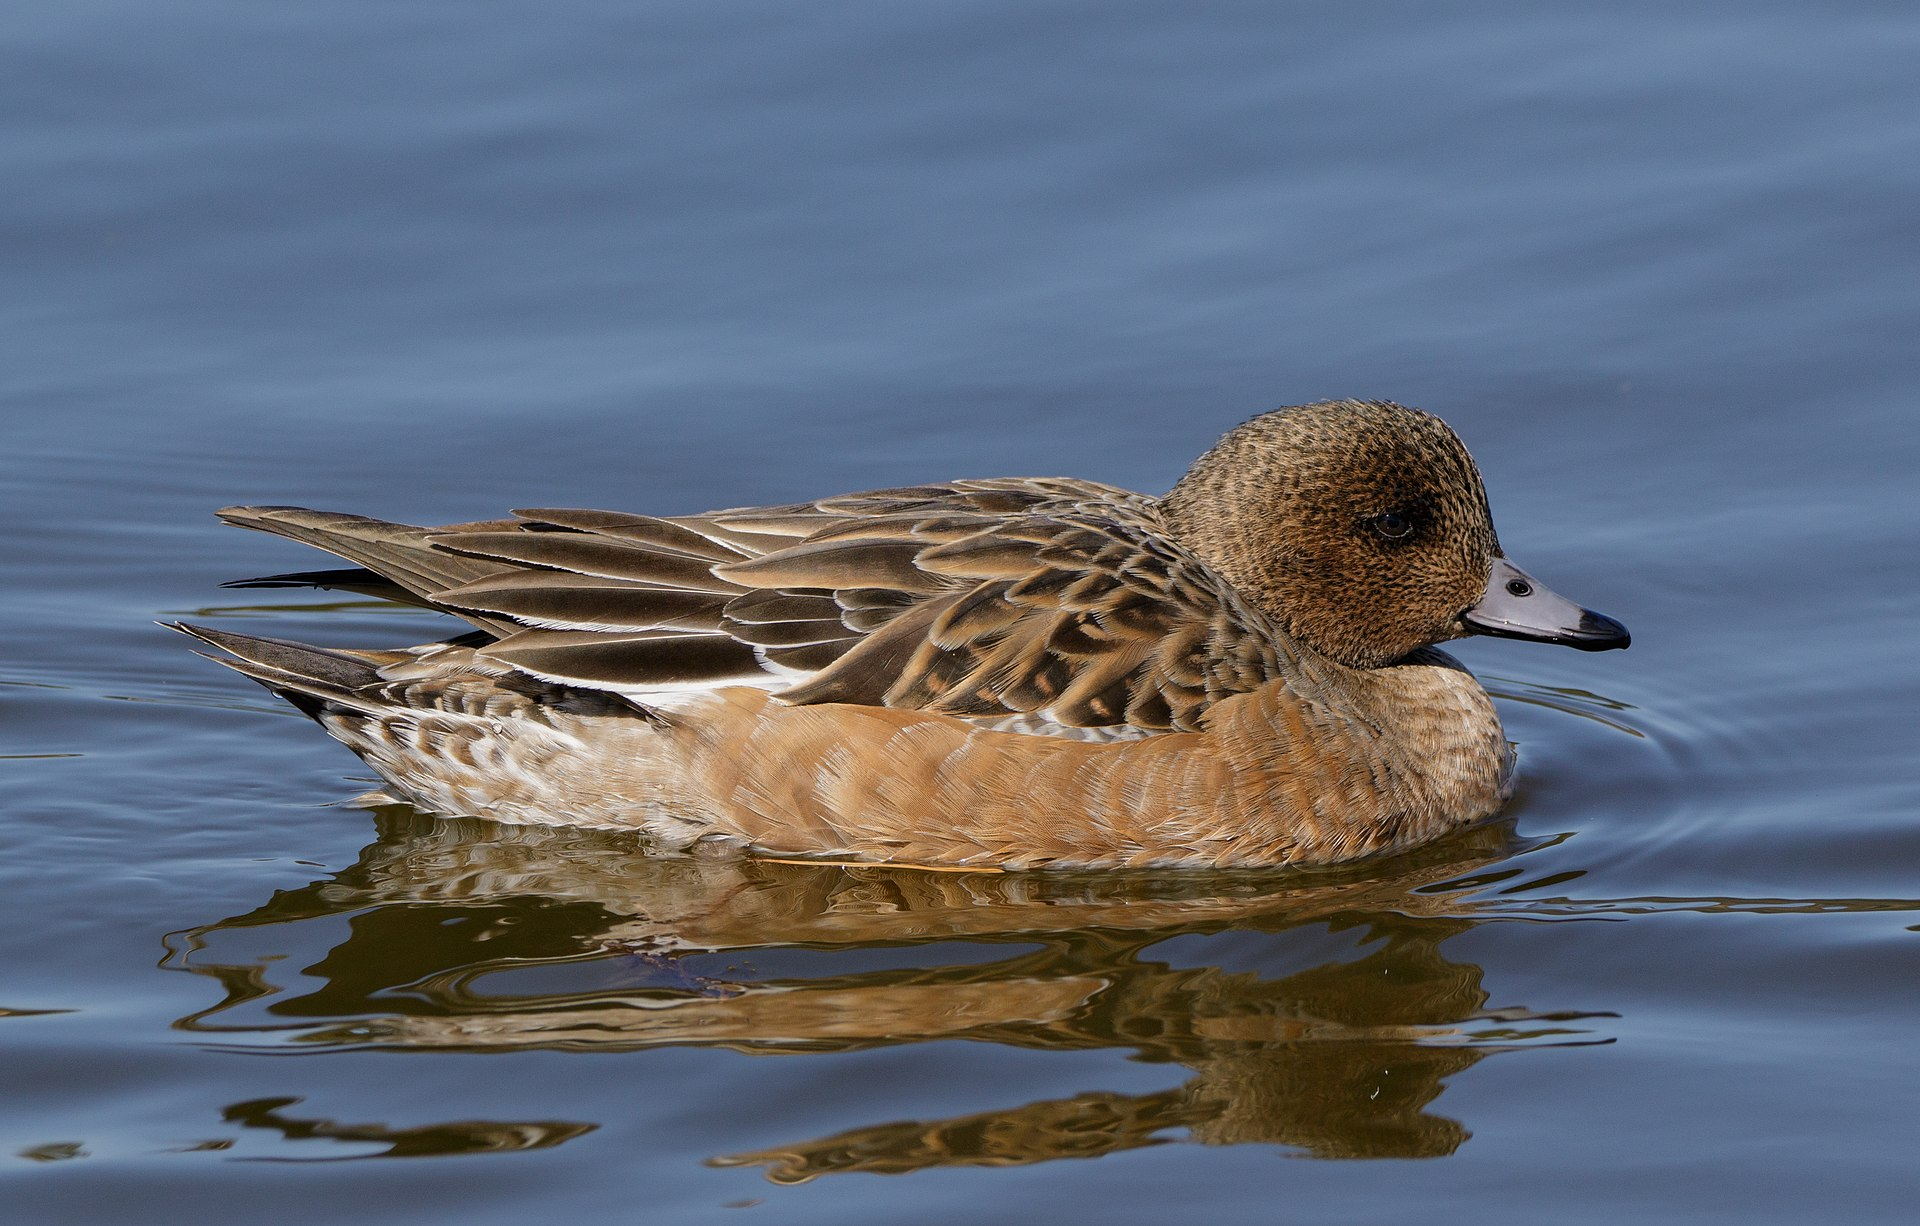
\includegraphics[width=0.8\linewidth, height=3.5cm, keepaspectratio]{Billeder/Dyr/Fugle/Aender/Svoemmeaender/pibeand_hun.jpg}%
      \end{minipage}
    }%
    \vspace{0.05em}
    \footnotesize Andrik øverst, and nederst
  \end{columns}
\end{frame}
% Eksempel: Indholdsframe om Spidsand (med to ikoner i højre margin via minipages)
\begin{frame}{%
  \begin{minipage}[t]{0.32\textwidth}
    Spidsand
  \end{minipage}%
  \hfill
  \begin{minipage}[t]{0.36\textwidth}
    \centering
    \footnotesize\textbf{Jagttid:} 1.\ september -- 31.\ december
  \end{minipage}%
  \hfill
  \begin{minipage}[t]{0.15\textwidth}
    \noindent\raggedleft
    
\includegraphics[width=0.5cm, height=0.5cm, keepaspectratio]{Billeder/Ikoner/star.png}%
    \hspace{0.2em}%
    
\includegraphics[width=0.5cm, height=0.5cm, keepaspectratio]{Billeder/Ikoner/star.png}
  \end{minipage}%
} % Ændret: Højre minipage nu med begge ikoner side om side
  \vspace{0.25em}
  \begin{columns}[T]
    % --- Venstre kolonne: Tekst ---
    \column{0.55\textwidth}
    \setlength{\parskip}{0.3em}
    \small
    \RaggedRight\textbf{\textit{Anas acuta}} – mellemstor svømmeand med slank kropsbygning \par

    \textbf{Udseende:} \\
    \quad – Andrik: chokoladefarvet hoved med hvid stribe i nakken, spids hale, hvidt bryst \\
    \quad – And: smal gråt næb, spids hale, lysebrun fjerdragt \par

    \textbf{Levesteder:} \\
    \quad – Kystnære engarealer

    \textbf{Føde:} \\
    \quad – Plantearter, kogleaks, smådyr \par

    \textbf{Udbredelse:} \\
    \quad – Hele Danmark \par

    \textbf{Træk/standfugl} \\
    \quad – Primært trækfugl \par

    % --- Højre kolonne: To billeder stablet over hinanden (større størrelse) ---
    \column{0.40\textwidth}
    \centering
    \fbox{%
      \begin{minipage}{\linewidth}
        \centering
        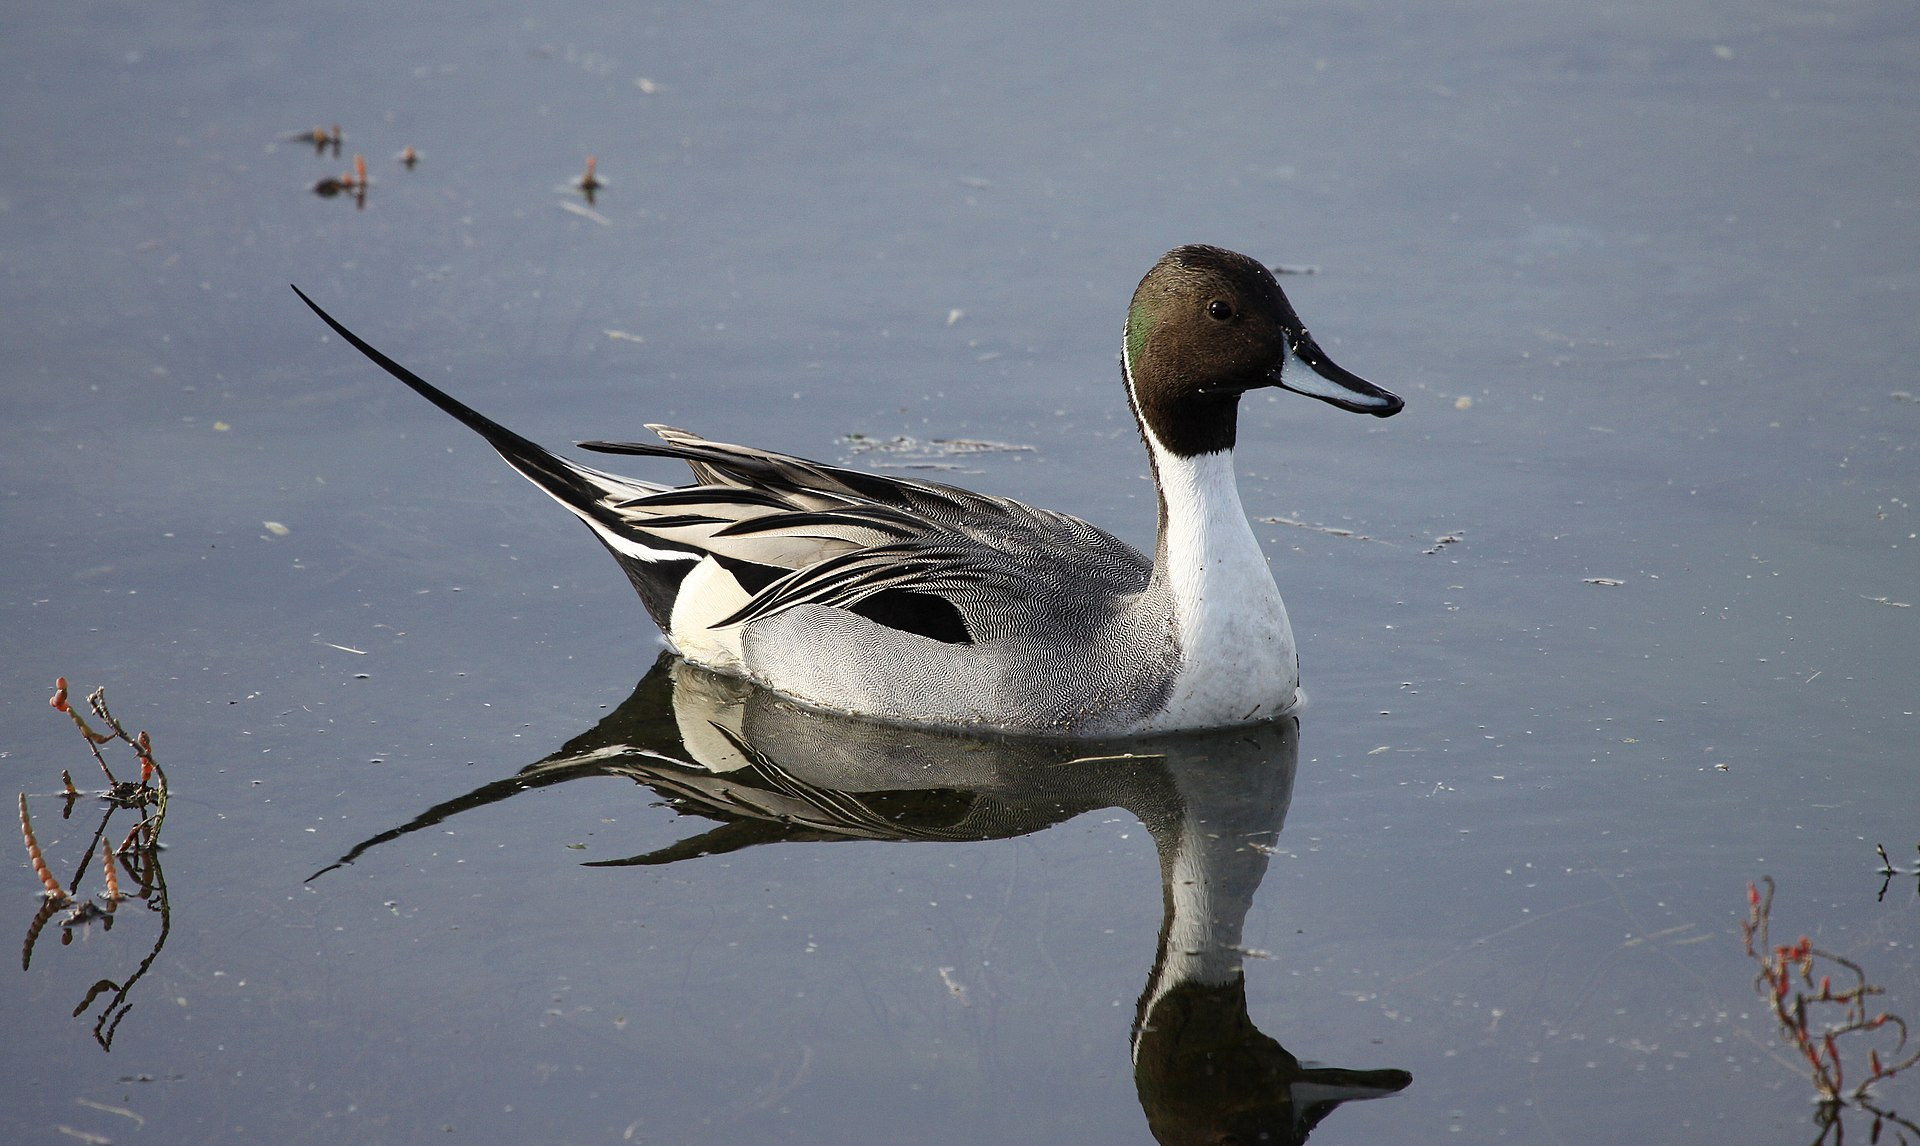
\includegraphics[width=0.8\linewidth, height=3.5cm, keepaspectratio]{Billeder/Dyr/Fugle/Aender/Svoemmeaender/spidsand_han.jpg}\\[0.5em]
        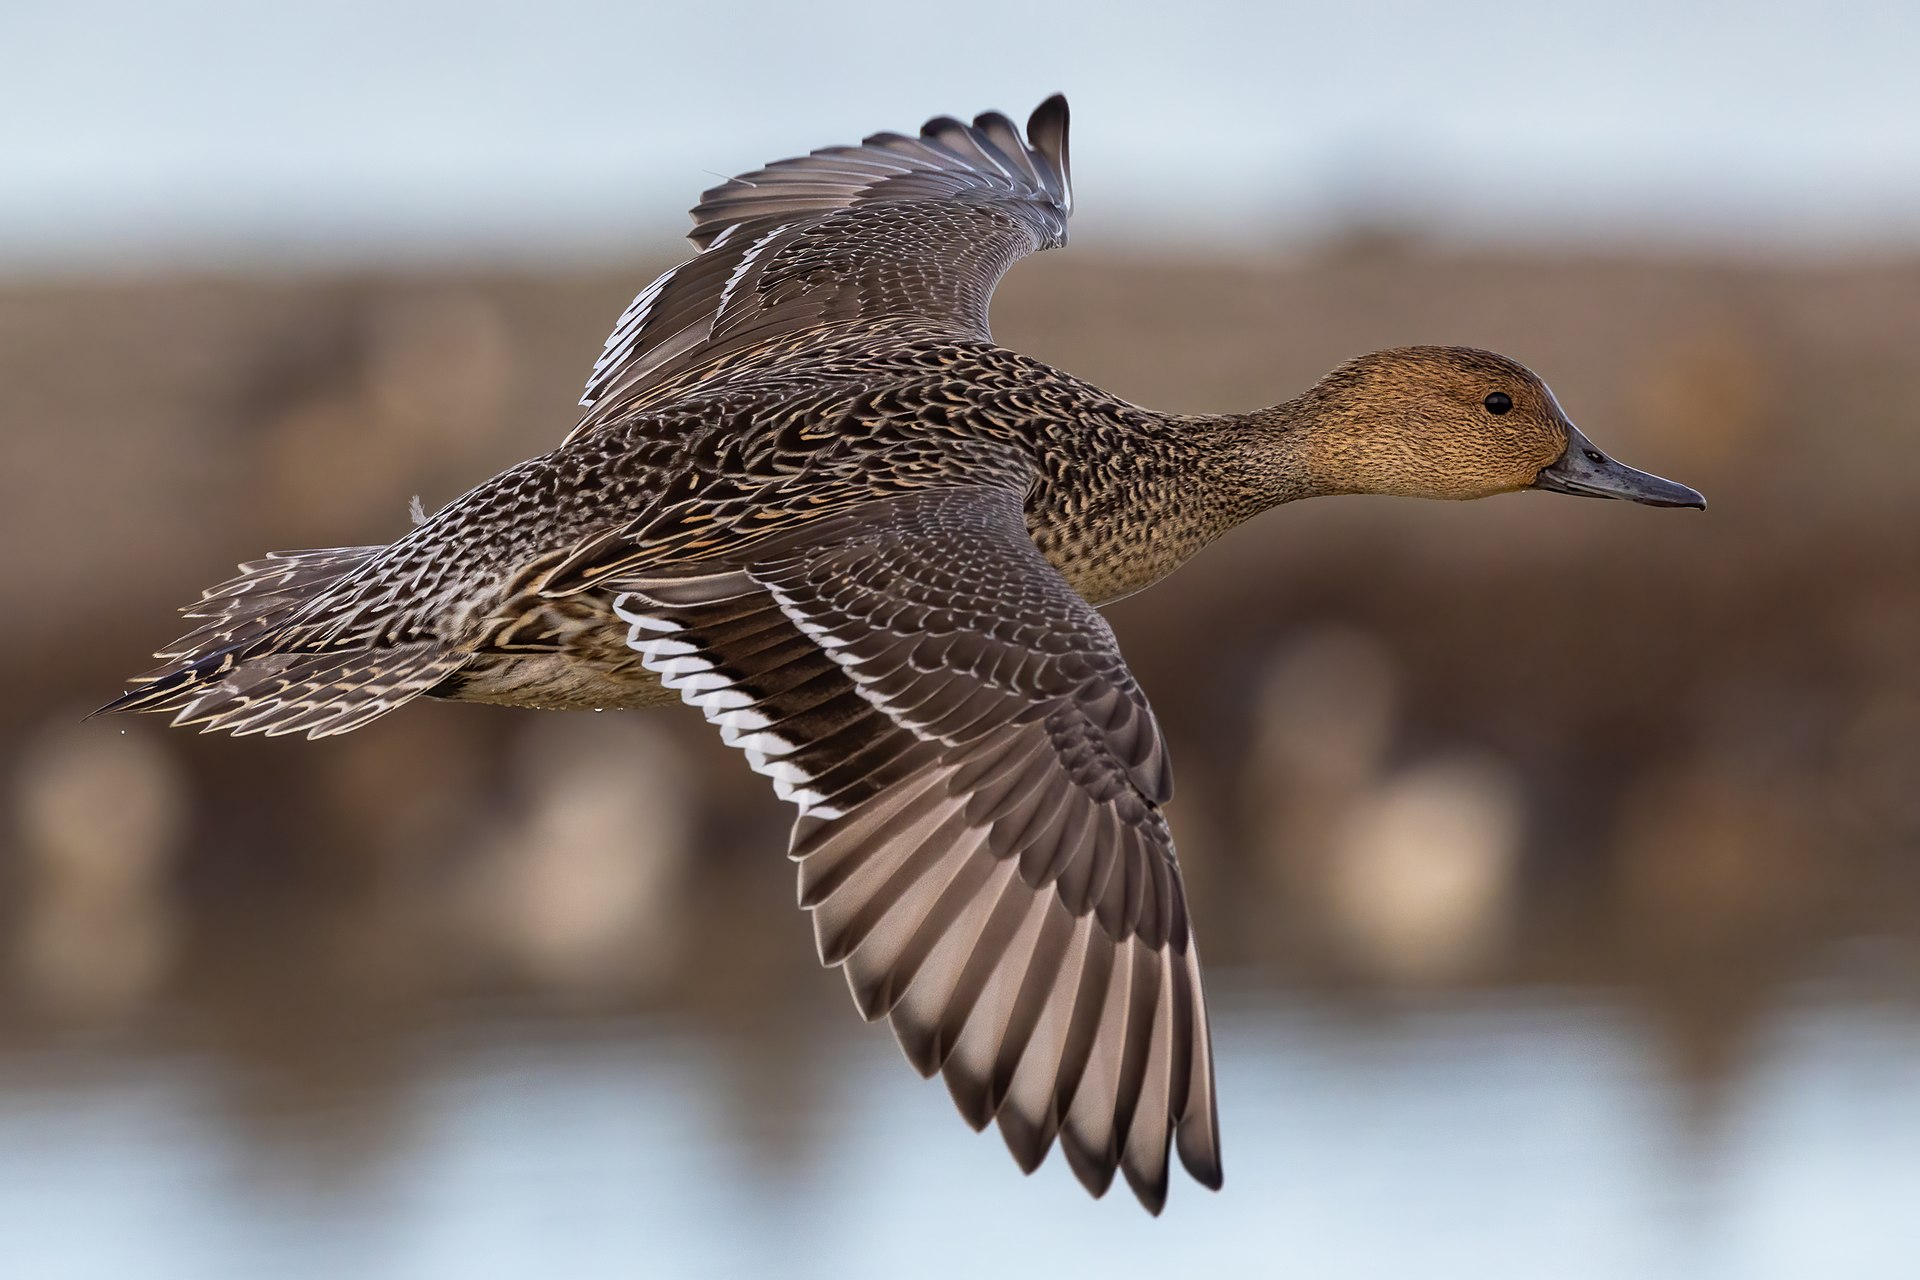
\includegraphics[width=0.8\linewidth, height=3.5cm, keepaspectratio]{Billeder/Dyr/Fugle/Aender/Svoemmeaender/spidsand_hun.jpg}%
      \end{minipage}
    }%
    \vspace{0.05em}
    \footnotesize Andrik øverst, and nederst
  \end{columns}
\end{frame}
%KRIKAND

% Eksempel: Indholdsframe om Krikand (med to ikoner i højre margin via minipages)
\begin{frame}{%
  \begin{minipage}[t]{0.32\textwidth}
    Krikand
  \end{minipage}%
  \hfill
  \begin{minipage}[t]{0.36\textwidth}
    \centering
    \footnotesize\textbf{Jagttid:} 1.\ september -- 31.\ december
  \end{minipage}%
  \hfill
  \begin{minipage}[t]{0.15\textwidth}
    \noindent\raggedleft
    
\includegraphics[width=0.5cm, height=0.5cm, keepaspectratio]{Billeder/Ikoner/star.png}%
    \hspace{0.2em}%
    
\includegraphics[width=0.5cm, height=0.5cm, keepaspectratio]{Billeder/Ikoner/star.png}
  \end{minipage}%
} % Ændret: Højre minipage nu med begge ikoner side om side
  \vspace{0.25em}
  \begin{columns}[T]
    % --- Venstre kolonne: Tekst ---
    \column{0.55\textwidth}
    \setlength{\parskip}{0.5em}
    \small
    \RaggedRight\textbf{\textit{Anas crecca}} – lille svømmeand, meget andræt i luften. \par

    \textbf{Udseende:} \\
    \quad – Andrik: rødbrunt hoved med grøn øjestribe. Louis Vuitton \\
    \quad – And: lille næb og grønlig fjerdragt \par

    \textbf{Levesteder:} \\
    \quad – Tilgroede vandhuller, moser og hedesøer

    \textbf{Føde:} \\
    \quad – Smådyr og planter \par

    \textbf{Udbredelse:} \\
    \quad – Hele Danmark \par

    \textbf{Træk/standfugl} \\
    \quad – Primært trækfugl \par

    % --- Højre kolonne: To billeder stablet over hinanden (større størrelse) ---
    \column{0.40\textwidth}
    \centering
    \fbox{%
      \begin{minipage}{\linewidth}
        \centering
        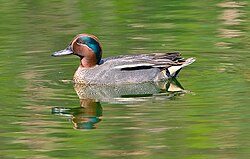
\includegraphics[width=0.8\linewidth, height=3.5cm, keepaspectratio]{Billeder/Dyr/Fugle/Aender/Svoemmeaender/krikand_han.jpg}\\[0.5em]
        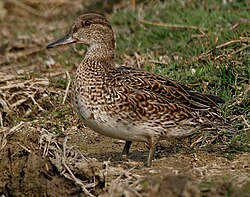
\includegraphics[width=0.8\linewidth, height=3.0cm, keepaspectratio]{Billeder/Dyr/Fugle/Aender/Svoemmeaender/krikand_hun.jpg}%
      \end{minipage}
    }%
    \vspace{0.05em}
    \footnotesize Andrik øverst, and nederst
  \end{columns}
\end{frame}
%  KNARAND

\begin{frame}{%
  \begin{minipage}[t]{0.32\textwidth}
    Knarand
  \end{minipage}%
  \hfill
  \begin{minipage}[t]{0.36\textwidth}
    \centering
    \footnotesize\textbf{Jagttid:} 1.\ september -- 31.\ december
  \end{minipage}%
  \hfill
  \begin{minipage}[t]{0.15\textwidth}
    \noindent\raggedleft
    
\includegraphics[width=0.5cm, height=0.5cm, keepaspectratio]{Billeder/Ikoner/star.png}%
  \end{minipage}%
} 
  \vspace{0.25em}
  \begin{columns}[T]
    % --- Venstre kolonne: Tekst ---
    \column{0.55\textwidth}
    \setlength{\parskip}{0.5em}
    \small
    \RaggedRight\textbf{\textit{Mareca strepera}} – mellemstor svømmeand også kaldet perlemorsand \par

    \textbf{Udseende:} \\
    \quad – Andrik: perlemorsfarvet bryst, lidt kedelig \\
    \quad – And: grålig, slangt guligt næb \par

    % --- Højre kolonne: To billeder stablet over hinanden ---
    \column{0.40\textwidth}
    \centering
    \fbox{%
      \begin{minipage}{\linewidth}
        \centering
        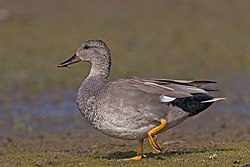
\includegraphics[width=0.8\linewidth, height=3.5cm, keepaspectratio]{Billeder/Dyr/Fugle/Aender/Svoemmeaender/knarand_han.jpg}\\[0.5em]
        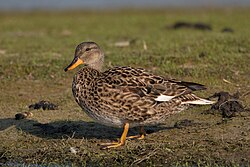
\includegraphics[width=0.8\linewidth, height=3.0cm, keepaspectratio]{Billeder/Dyr/Fugle/Aender/Svoemmeaender/knarand_hun.jpg}%
      \end{minipage}
    }%
    \vspace{0.05em}
    \footnotesize Andrik øverst, and nederst
  \end{columns}
\end{frame}
%   ATLINGAND

\begin{frame}{%
  \begin{minipage}[t]{0.32\textwidth}
    Atlingand
  \end{minipage}%
  \hfill
  \begin{minipage}[t]{0.36\textwidth}
    \centering
    \footnotesize\textbf{Jagttid:} 1.\ september -- 31.\ december
  \end{minipage}%
  \hfill
  \begin{minipage}[t]{0.15\textwidth}
    \noindent\raggedleft
    
\includegraphics[width=0.5cm, height=0.5cm, keepaspectratio]{Billeder/Ikoner/star.png}%
  \end{minipage}%
} 
  \vspace{0.25em}
  \begin{columns}[T]
    % --- Venstre kolonne: Tekst ---
    \column{0.55\textwidth}
    \setlength{\parskip}{0.5em}
    \small
    \RaggedRight\textbf{\textit{Anas querquedula}} – lille svømmeand kan forveksles med krikand \par

    \textbf{Udseende:} \\
    \quad – Andrik: brunt hovede med hvid stribe, kraftigt langt mørkt næb \\
    \quad – And: beige hage, kraftig langt mørkt næb \par

    % --- Højre kolonne: To billeder stablet over hinanden ---
    \column{0.40\textwidth}
    \centering
    \fbox{%
      \begin{minipage}{\linewidth}
        \centering
        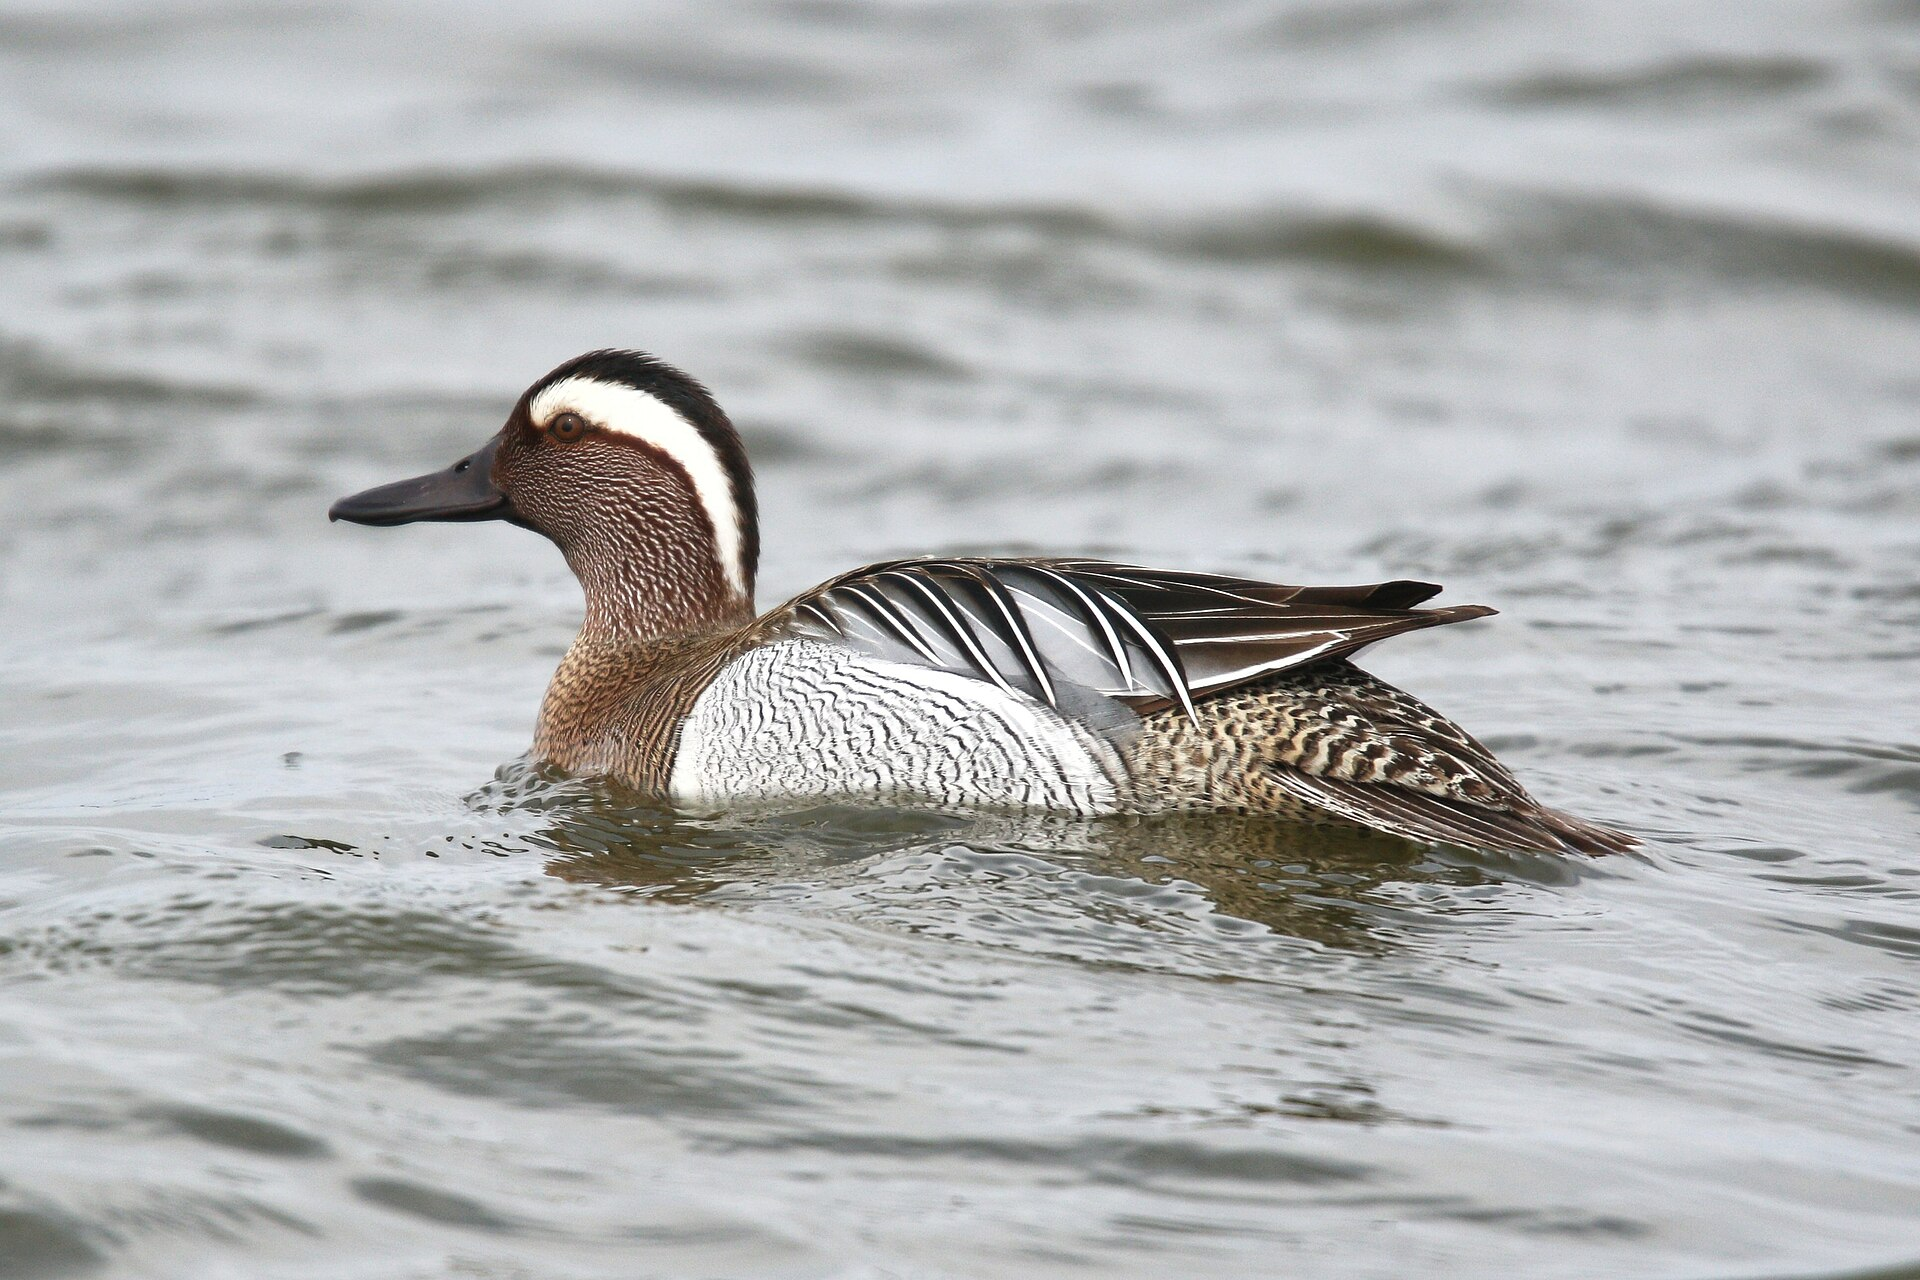
\includegraphics[width=0.8\linewidth, height=3.5cm, keepaspectratio]{Billeder/Dyr/Fugle/Aender/Svoemmeaender/atlingand_han.jpg}\\[0.5em]
        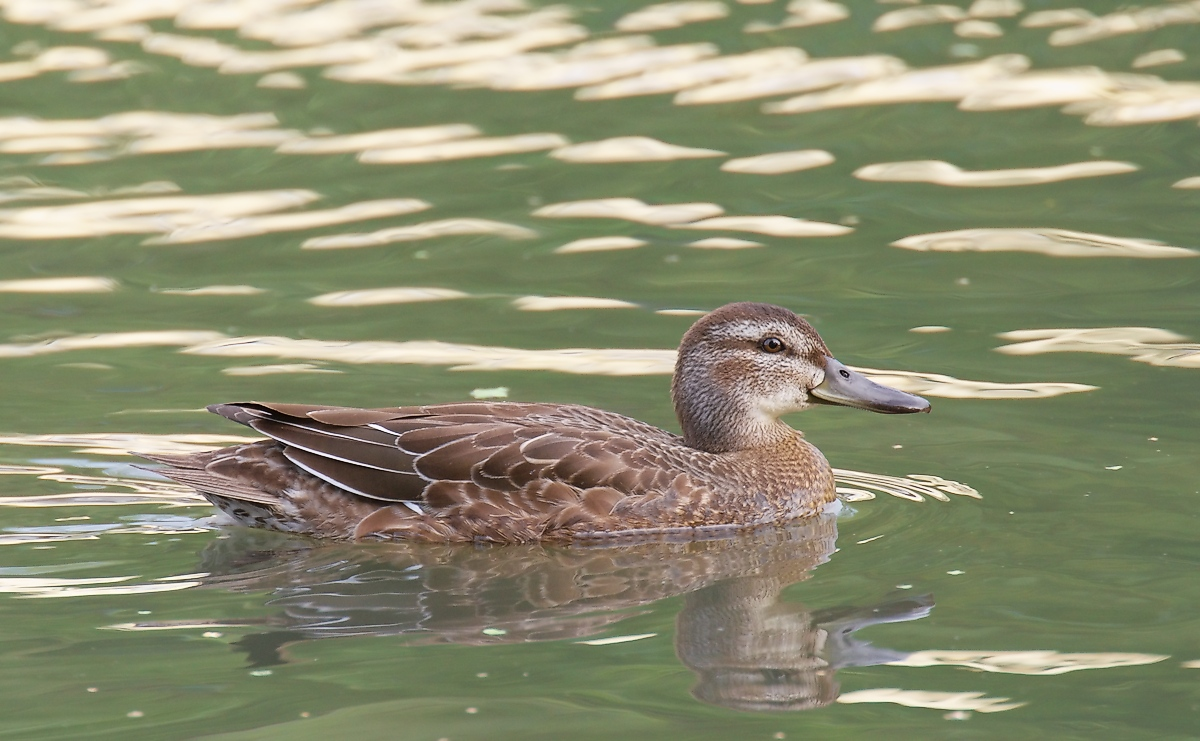
\includegraphics[width=0.8\linewidth, height=3.0cm, keepaspectratio]{Billeder/Dyr/Fugle/Aender/Svoemmeaender/atlingand_hun.jpg}%
      \end{minipage}
    }%
    \vspace{0.05em}
    \footnotesize Andrik øverst, and nederst
  \end{columns}
\end{frame}
%SKEAND

% Eksempel: Indholdsframe om Skeand (med én stjerne i højre margin)
\begin{frame}{%
  \begin{minipage}[t]{0.32\textwidth}
    Skeand
  \end{minipage}%
  \hfill
  \begin{minipage}[t]{0.36\textwidth}
    \centering
    \footnotesize\textbf{Jagttid:} 1.\ september -- 31.\ december
  \end{minipage}%
  \hfill
  \begin{minipage}[t]{0.15\textwidth}
    \noindent\raggedleft
    
\includegraphics[width=0.55cm, height=0.55cm, keepaspectratio]{Billeder/Ikoner/star.png}%
  \end{minipage}%
} 
  \vspace{0.25em}
  \begin{columns}[T]
    % --- Venstre kolonne: Tekst ---
    \column{0.55\textwidth}
    \setlength{\parskip}{0.5em}
    \small
    \RaggedRight\textbf{\textit{Anas clypeata}} – mellemstor svømmeand med meget karakteristisk næb \par

    \textbf{Udseende:} \\
    \quad – Andrik: stort skeformet næb \\
    \quad – And: stort skeformet næb \par

    

    % --- Højre kolonne: To billeder stablet over hinanden ---
    \column{0.40\textwidth}
    \centering
    \fbox{%
      \begin{minipage}{\linewidth}
        \centering
        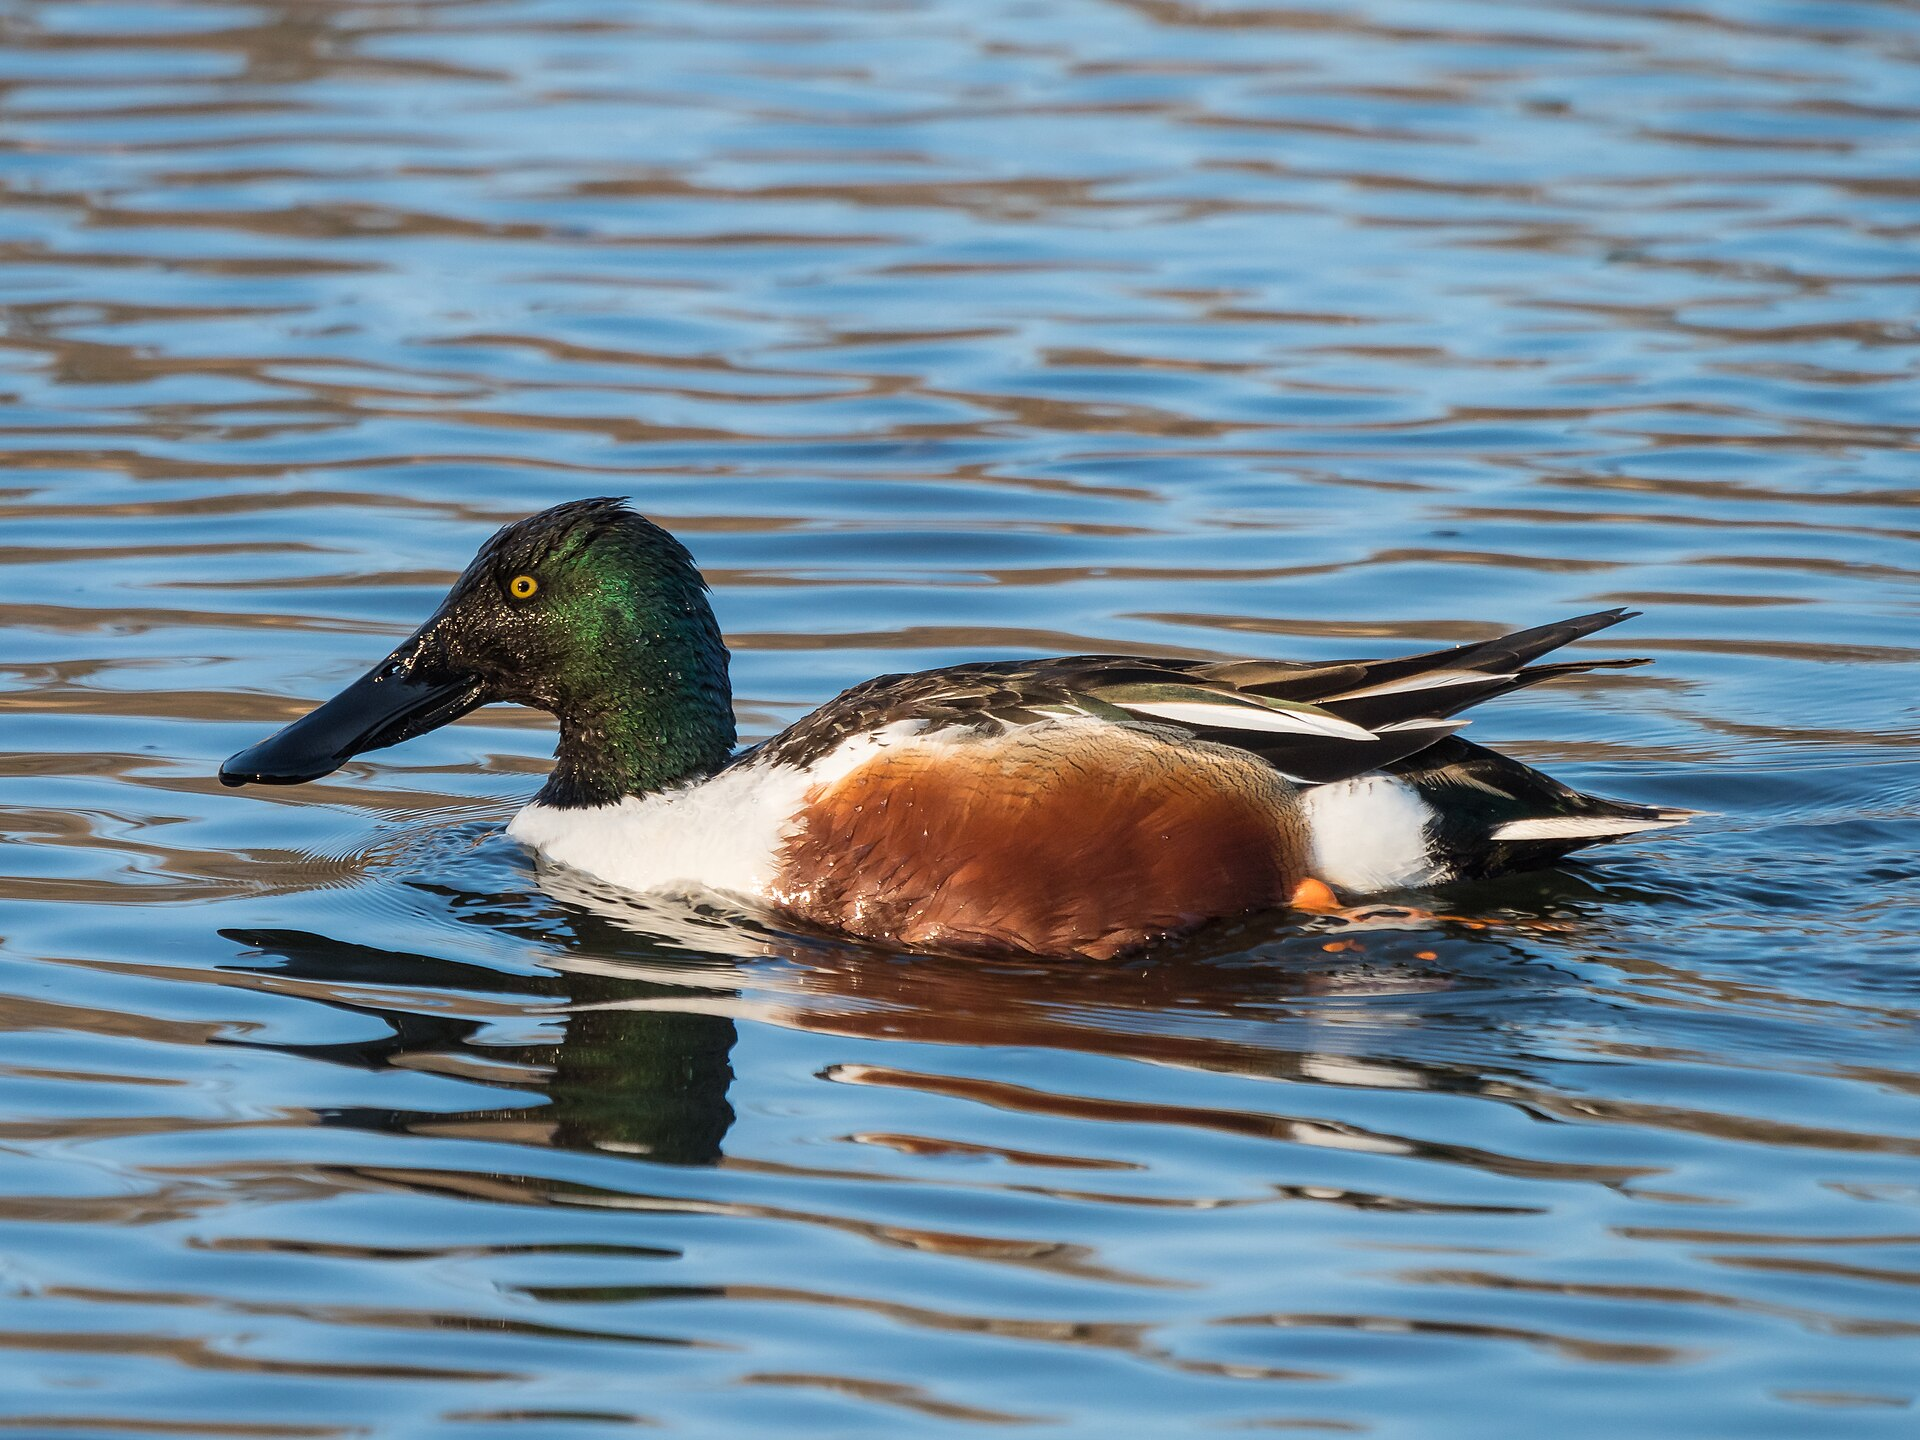
\includegraphics[width=0.8\linewidth, height=3cm, keepaspectratio]{Billeder/Dyr/Fugle/Aender/Svoemmeaender/skeand_han.jpg}\\[0.5em]
        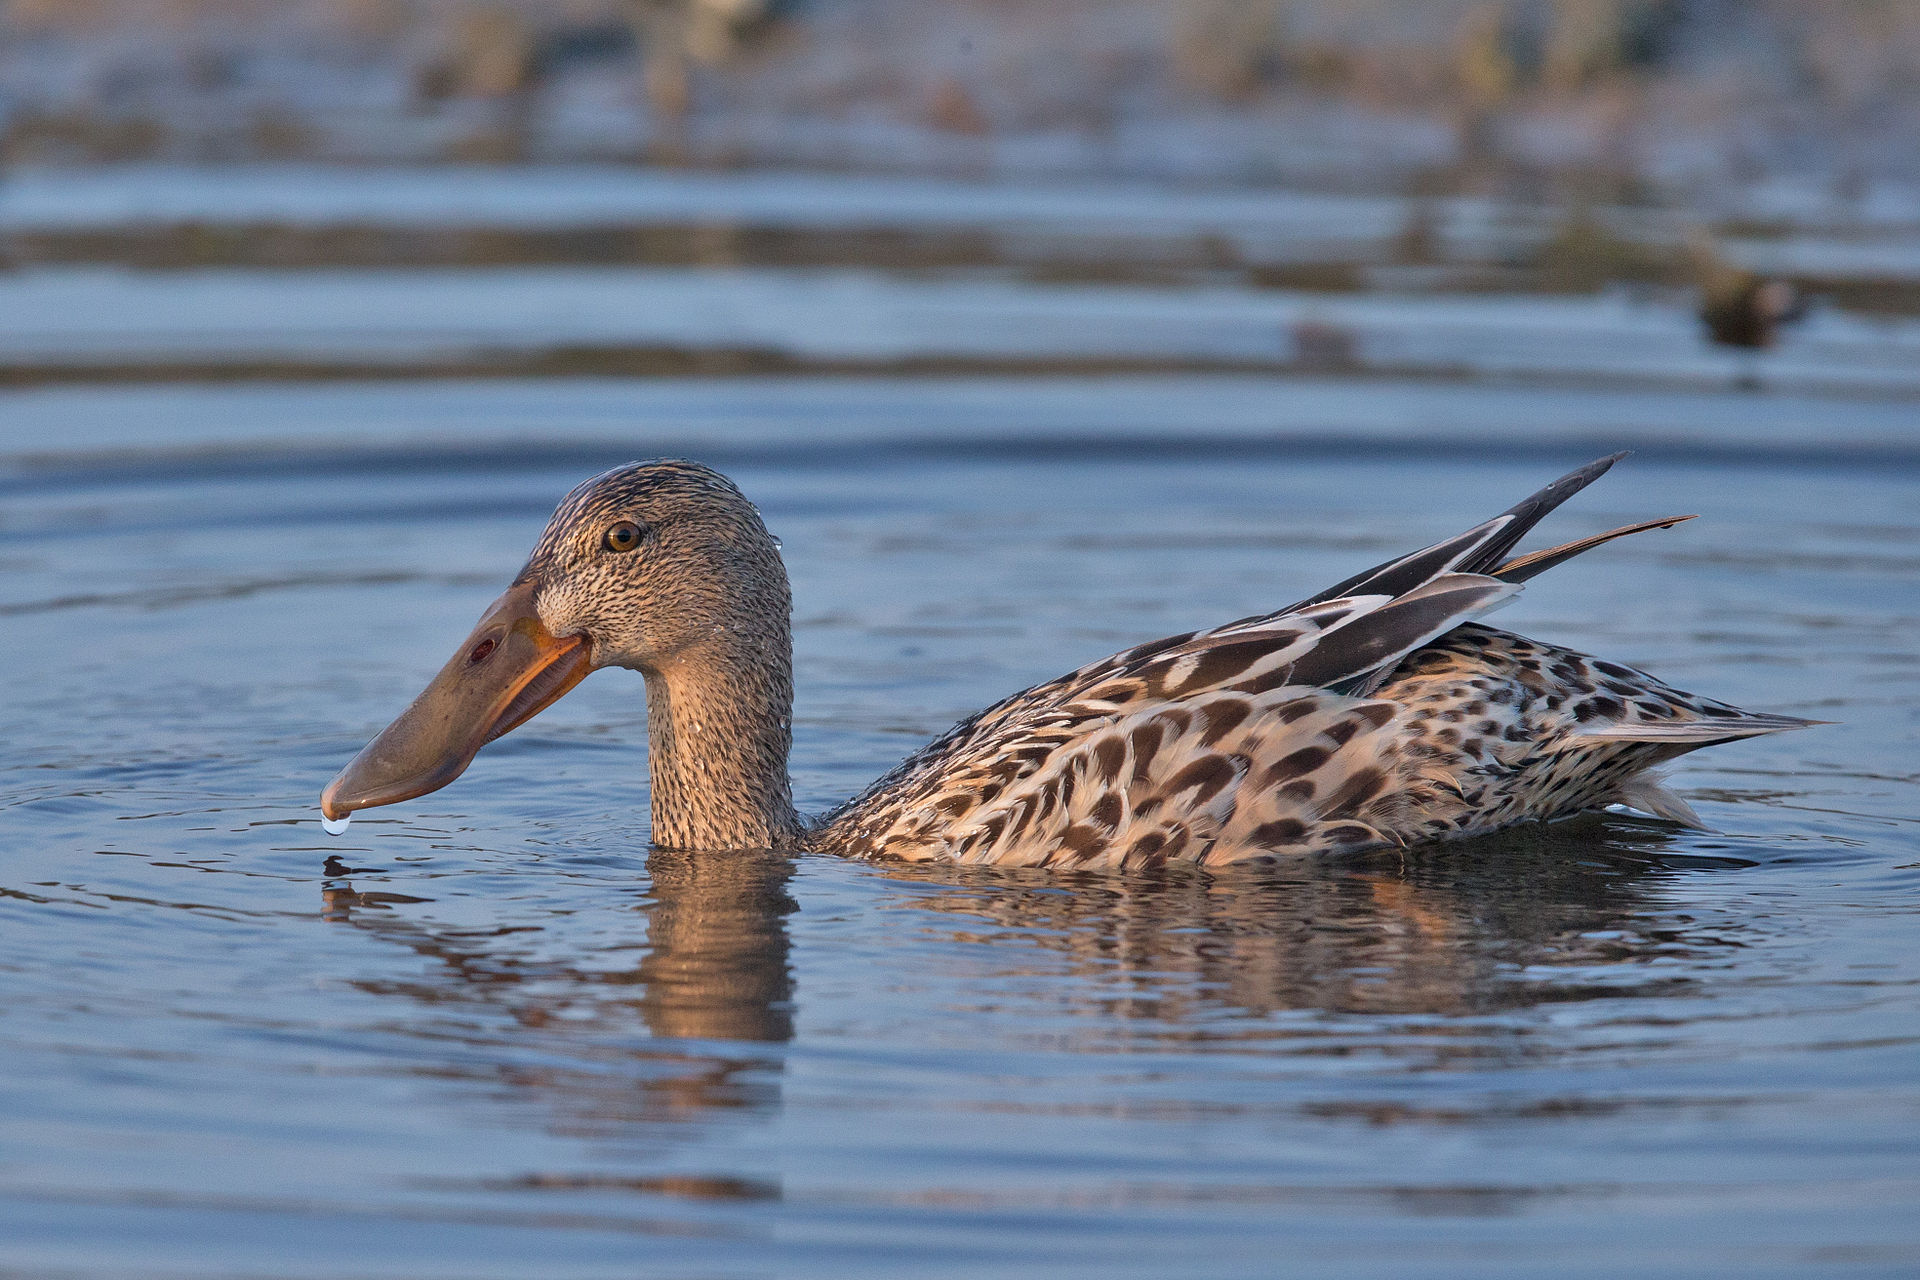
\includegraphics[width=0.8\linewidth, height=3cm, keepaspectratio]{Billeder/Dyr/Fugle/Aender/Svoemmeaender/skeand_hun.jpg}%
      \end{minipage}
    }%
    \vspace{0.05em}
    \footnotesize Andrik øverst, and nederst
  \end{columns}
\end{frame}

\end{document}